\documentclass[a4paper,11pt]{book}
%\documentclass[a4paper,twoside,11pt,titlepage]{book}
\usepackage{listings}
\usepackage[utf8]{inputenc}
\usepackage[spanish]{babel}
\usepackage{eurosym}


\decimalpoint
\usepackage{dcolumn}
\newcolumntype{.}{D{.}{\esperiod}{-1}}
\makeatletter
\addto\shorthandsspanish{\let\esperiod\es@period@code}
\makeatother


%\usepackage[chapter]{algorithm}
\RequirePackage{verbatim}
%\RequirePackage[Glenn]{fncychap}
\usepackage{fancyhdr}
\usepackage{graphicx}
\usepackage{afterpage}

\usepackage{longtable}

\usepackage[pdfborder={000}]{hyperref} %referencia


\newcommand{\myTitle}{ArduBand\xspace}
\newcommand{\myDegree}{Grado en Ingeniería Informática\xspace}
\newcommand{\myName}{Israel Blancas Álvarez\xspace}
\newcommand{\myProf}{Samuel Francisco Romero García\xspace}
\newcommand{\myFaculty}{Escuela Técnica Superior de Ingenierías Informática y de
Telecomunicación\xspace}
\newcommand{\myFacultyShort}{E.T.S. de Ingenierías Informática y de
Telecomunicación\xspace}
\newcommand{\myDepartment}{Departamento de Arquitectura y Tecnología de Computadores\xspace}
\newcommand{\myUni}{\protect{Universidad de Granada}\xspace}
\newcommand{\myLocation}{Granada\xspace}
\newcommand{\myTime}{\today\xspace}
\newcommand{\myVersion}{Version 0.1\xspace}


\hypersetup{
pdfauthor = {\myName Israel Blancas Álvarez},
pdftitle = {\myTitle ArduBand},
pdfsubject = {},
pdfkeywords = {ZigBee, Metrónomo, Arduino, WSN, XBee, Android},
pdfcreator = {LaTex},
pdfproducer = {pdflatex}
}

%\hyphenation{}


%\usepackage{doxygen/doxygen}
%\usepackage{pdfpages}
\usepackage{url}
\usepackage{colortbl,longtable}
\usepackage[stable]{footmisc}
%\usepackage{index}


%\usepackage[style=long, cols=2,border=plain,toc=true,number=none]{glossary}
% \makeglossary

% Definición de comandos que me son tiles:
%\renewcommand{\indexname}{Índice alfabético}
%\renewcommand{\glossaryname}{Glosario}

\pagestyle{fancy}
\fancyhf{}
\fancyhead[LO]{\leftmark}
\fancyhead[RE]{\rightmark}
\fancyhead[RO,LE]{\textbf{\thepage}}
\renewcommand{\chaptermark}[1]{\markboth{\textbf{#1}}{}}
\renewcommand{\sectionmark}[1]{\markright{\textbf{\thesection. #1}}}

\setlength{\headheight}{1.5\headheight}

\newcommand{\HRule}{\rule{\linewidth}{0.5mm}}
%Definimos los tipos teorema, ejemplo y definición podremos usar estos tipos
%simplemente poniendo \begin{teorema} \end{teorema} ...
\newtheorem{teorema}{Teorema}[chapter]
\newtheorem{ejemplo}{Ejemplo}[chapter]


\definecolor{gray97}{gray}{.97}
\definecolor{gray75}{gray}{.75}
\definecolor{gray45}{gray}{.45}
\definecolor{gray30}{gray}{.94}

\lstset{ frame=Ltb,
     framerule=0.5pt,
     aboveskip=0.5cm,
     framextopmargin=3pt,
     framexbottommargin=3pt,
     framexleftmargin=0.1cm,
     framesep=0pt,
     rulesep=.4pt,
     backgroundcolor=\color{gray97},
     rulesepcolor=\color{black},
     %
     stringstyle=\ttfamily,
     showstringspaces = false,
     basicstyle=\scriptsize\ttfamily,
     commentstyle=\color{gray45},
     keywordstyle=\bfseries,
     %
     numbers=left,
     numbersep=6pt,
     numberstyle=\tiny,
     numberfirstline = false,
     breaklines=true,
   }

\lstnewenvironment{listing}[1][]
   {\lstset{#1}\pagebreak[0]}{\pagebreak[0]}

\lstdefinestyle{CodigoC}
   {
	basicstyle=\scriptsize,
	frame=single,
	language=C,
	numbers=left
   }

\lstdefinestyle{Consola}
   {basicstyle=\scriptsize\bf\ttfamily,
    backgroundcolor=\color{gray30},
    frame=single,
    numbers=none
   }


\newcommand{\bigrule}{\titlerule[0.5mm]}


%Para conseguir que en las páginas en blanco no ponga cabeceras
\makeatletter
\def\clearpage{%
  \ifvmode
    \ifnum \@dbltopnum =\m@ne
      \ifdim \pagetotal <\topskip
        \hbox{}
      \fi
    \fi
  \fi
  \newpage
  \thispagestyle{empty}
  \write\m@ne{}
  \vbox{}
  \penalty -\@Mi
}
\makeatother

\usepackage{pdfpages}
\begin{document}
\begin{titlepage}
 
 
\newlength{\centeroffset}
\setlength{\centeroffset}{-0.5\oddsidemargin}
\addtolength{\centeroffset}{0.5\evensidemargin}
\thispagestyle{empty}

\noindent\hspace*{\centeroffset}\begin{minipage}{\textwidth}

\centering

\includegraphics[width=0.9\textwidth]{imagenes/logo_ugr.jpg}\\[1.4cm]

\textsc{ \Large TRABAJO FIN DE GRADO\\[0.2cm]}
\textsc{ INGENIERÍA EN ...}\\[1cm]
% Upper part of the page
% 
% Title
{\Huge\bfseries Titulo del Proyecto\\
}
\noindent\rule[-1ex]{\textwidth}{3pt}\\[3.5ex]
{\large\bfseries Subtitulo del Proyecto}
\end{minipage}

\vspace{2.5cm}
\noindent\hspace*{\centeroffset}\begin{minipage}{\textwidth}
\centering

\textbf{Autor}\\ {Nombre Apellido1 Apellido2 (alumno)}\\[2.5ex]
\textbf{Directores}\\
{Nombre Apellido1 Apellido2 (tutor1)\\
Nombre Apellido1 Apellido2 (tutor2)}\\[2cm]

\includegraphics[width=0.3\textwidth]{imagenes/etsiit_logo.png}\\[0.1cm]
\textsc{Escuela Técnica Superior de Ingenierías Informática y de Telecomunicación}\\
\textsc{---}\\
Granada, mes de 201
\end{minipage}
%\addtolength{\textwidth}{\centeroffset}
%\vspace{\stretch{2}}
\end{titlepage}



\chapter*{}
%\thispagestyle{empty}
%\cleardoublepage

%\thispagestyle{empty}

\begin{titlepage}
 
 
\setlength{\centeroffset}{-0.5\oddsidemargin}
\addtolength{\centeroffset}{0.5\evensidemargin}
\thispagestyle{empty}

\noindent\hspace*{\centeroffset}\begin{minipage}{\textwidth}

\centering
%
\includegraphics[width=0.9\textwidth]{imagenes/logo_ugr.jpg}\\[1.4cm]

%\textsc{ \Large PROYECTO FIN DE CARRERA\\[0.2cm]}
%\textsc{ INGENIERÍA EN INFORMÁTICA}\\[1cm]
% Upper part of the page
% 

 \vspace{3.3cm}

%si el proyecto tiene logo poner aquí

\includegraphics{imagenes/logo.png} 
 \vspace{0.5cm}

% Title

{\Huge\bfseries Título del proyecto\\
}
\noindent\rule[-1ex]{\textwidth}{3pt}\\[3.5ex]
{\large\bfseries Subtítulo del proyecto.\\[4cm]}
\end{minipage}

\vspace{2.5cm}
\noindent\hspace*{\centeroffset}\begin{minipage}{\textwidth}
\centering

\textbf{Autor}\\ {Nombre Apellido1 Apellido2 (alumno)}\\[2.5ex]
\textbf{Directores}\\
{Nombre Apellido1 Apellido2 (tutor1)\\
Nombre Apellido1 Apellido2 (tutor2)}\\[2cm]
%
\includegraphics[width=0.15\textwidth]{imagenes/tstc.png}\\[0.1cm]
%\textsc{Departamento de Teoría de la Señal, Telemática y Comunicaciones}\\
%\textsc{---}\\
%Granada, mes de 201
\end{minipage}
%\addtolength{\textwidth}{\centeroffset}
\vspace{\stretch{2}}

 
\end{titlepage}





\cleardoublepage
\thispagestyle{empty}

\begin{center}
{\large\bfseries ArduBand: sistema  \textit{wearable} para sincronización de bandas de música}\\
\end{center}
\begin{center}
Israel Blancas Álvarez\\
\end{center}

%\vspace{0.7cm}
\noindent{\textbf{Palabras clave}: ZigBee, Metrónomo, Arduino, WSN, XBee, Android}\\

\vspace{0.7cm}
\noindent{\textbf{Resumen}}\\
En el presente trabajo, el lector podrá encontrar cómo se ha desarrollado un sistema
\textit{wearable} que, mediante vibración, facilita a los intérpretes de una banda de
música seguir el mismo tempo. De esta forma, se ayudará a que todos los miembros del conjunto
sigan el mismo pulso y puedan mantenerlo constante durante toda la ejecución.\\

Esta necesidad ha despertado el interés de algunas compañías, que han desarrollado como el
llamado ``Body Beat", de la marca ``Peterson" que, a pesar de su gran abanico de funciones,
no ha tenido el éxito esperado en el mercado al tener elevado coste. Un sistema que hiciese las
veces de metrónomo wireless (característica principal y más atrayente del artículo antes mencionado)
a un precio menor atraería a muchos más clientes.\\

Para que todos los integrantes de la agrupación puedan llevar el mismo pulso, se ha creado una red
inalámbrica de sensores (WSN) que permite la sincronización de los aparatos que portan todos los músicos.
La red de sensores ha sido concebida utilizando la implementación de ZigBee propuesta por la empresa “Digi
International”, mientras la lógica de los circuitos se ha puesto en manos de la plataforma hardware Arduino
(utilizándose diversas versiones del mismo).\\

El tipo de red que forman los dispositivos ``XBee ZigBee" es de tipo malla pero, utilizando la configuración
de las motas, se ha pasado a tener una topología de estrella. Dispone de dos tipos de  \textit{wearables}:
  \begin{itemize}
  \item Director: su mota juega el papel de ``coordinador" de la red. Es quien crea la red y establece los caminos que deben seguir las comunicaciones que haya en la red. Además de la comunicación con los otros elementos del sistema, tiene la opción de conectar, a través de Bluetooth, con un dispositivo Android.
  \item Músico: contiene una mota del tipo ``dispositivo final". Simplemente, recibe (del dispositivo ``director") el tempo con el que el micromotor vibrador debe activarse (además, al llegar el paquete con la traza de datos, se sincroniza con el resto de dispositivos de la red, de forma que todos vibren a la vez).
  \end{itemize}

Como se comentaba cuando se hablaba del dispositivo del director, se puede conectar
con un dispositivo móvil Android. Es necesario que el director indique el tempo que el
sistema debe marcar a los músicos, esta aplicación móvil es la que transfiere al controlador la
velocidad a la que debe compaginar a los intérpretes (para evitar sobrecargar la red, se hace una
coordinación cada cierto tiempo -por si hubiera habido retrasos en la organización inicial- y cada
dispositivo subdivide en función del tempo que se le ha enviado). Buscando facilitar al usuario la utilización
de esta tecnología, se ha desarrollado tanto una aplicación para teléfonos móviles, como para smartwatches
que funcionen con el sistema operativo ``Android Wear".\\

Una vez desarrollada la base del sistema, es posible crear nuevas funcionalidades como la instalación de un
sensor de vibración que permita a los percusionistas obtener retroalimentación para saber si los intérpretes
están ejecutando la partitura siguiendo el tiempo marcado o la posibilidad de pasar lista (conociendo qué sensores
se encuentran activos en la red).\\

\cleardoublepage


\thispagestyle{empty}


\begin{center}
{\large\bfseries ArduBand: wearable system to synchronize music bands}\\
\end{center}
\begin{center}
Israel Blancas\\
\end{center}

%\vspace{0.7cm}
\noindent{\textbf{Keywords}: ZigBee, Metronome, Arduino, WSN, XBee, Android}\\

\vspace{0.7cm}
\noindent{\textbf{Abstract}}\\

One of the principles of engineering is creating solutions to the problems of users.
In this dissertation, the reader will be able to find how a wearable system has been developed
helping musicians to go on the same “tempo” through vibration while they are playing music.
This device sends the same pulse to all musicians and keep the “tempo” constant.\\

Some companies have developed similar systems. For example, Peterson created an item called “Body Beat”.
It has a big range of functions and odds but it is too expensive for the majority of musicians. One device
cheaper than it only with synchronization functions (the most important ability of this system) could attract
more buyers. Furthermore, to create a free and open hardware platform could interest other developers to improve
the functionality of this product (helping musicians, music teachers and other music professionals to play music
with a better quality).\\

All music band’s components need to have the same pulse (if each instrumentalist had a different pulse, each
one would read his score in a different speed and it would be a problem). It is possible because it has been
created using a wireless sensor network (they enable communication with a very low energy cost). Then, when all
nodes are synchronized, they know when they have to start the vibrations. But they do not have to be vibrating all
time. They have to vibrate constantly as many times as the director said (for example, if compasses are of 4/4 and
tempo 60 bpm -Beats Per Minute-, each node will vibrate 1 time per second).\\

This network has been deployed using ZigBee implementation of the “Digi International” company. Also, circuit logic
has been put into operation using the hardware platform called Arduino (various versions of this, like Arduino Lilypad,
Arduino Uno or Arduino Leonardo).\\

In the following pages , it is explained in more detail why certain decisions have been taken (some experiments in
time between node's communications, explanations about XBee communication packets...).\\

XBee Zigbee’s devices are organized in mesh network but, changing each node’s configuration, we have now a network with
star topology. There are two kinds of wearables:
  \begin{itemize}
  \item Music director: it is the coordinator of network. It is who start the network and establish the paths of communication packets between all nodes. In addition, it is able to send data to every node and receive data from an Android device via Bluetooth. Only one in each network.
  \item Musician: it is composed of an “end device” node. It receives (from “music director device”) data (which contains “tempo”). Arduino takes this tempo and performs calculations to decide when it has to activate or deactivate a vibration motor (this motor helps musician to keep track of the correct pulse). There is one for each musician (in network, there will be as nodes as musicians).
  \end{itemize}


Director’s device can be connected to an Android device (which could be a smartphone or a smartwatch,
because one application has been developed to each one). This application allows director to indicate music’s
``tempo" and each application was developed using Google’s recommendations about design (Material Design principles).\\

Taking this base, it is possible to create new functions such as installing a vibration sensors in drums to measure the
tempo of the band and provide a feedback to the director. Another possibility could be rollcalling at the band (only it
is necessary show what nodes are in the network at the moment).\\


\chapter*{}
\thispagestyle{empty}

\noindent\rule[-1ex]{\textwidth}{2pt}\\[4.5ex]

Yo, \textbf Israel Blancas Álvarez, alumno de la titulación Grado de Ingeniería Informática de la \textbf{Escuela Técnica Superior
de Ingenierías Informática y de Telecomunicación de la Universidad de Granada}, con DNI XXXXXXXXX, autorizo la
ubicación de la siguiente copia de mi Trabajo Fin de Grado en la biblioteca del centro para que pueda ser
consultada por las personas que lo deseen.

\vspace{6cm}

\noindent Fdo: Israel Blancas Álvarez

\vspace{2cm}

\begin{flushright}
Granada a 1 de julio de 2015.
\end{flushright}


\chapter*{}
\thispagestyle{empty}

\noindent\rule[-1ex]{\textwidth}{2pt}\\[4.5ex]

D. \textbf{Samuel Francisco Romero García}, Profesor del Área de Arquitectura y Tecnología de Computadores del Departamento Arquitectura y Tecnología de Computadores de la Universidad de Granada.

\vspace{0.5cm}


\vspace{0.5cm}

\textbf{Informa:}

\vspace{0.5cm}

Que el presente trabajo, titulado \textit{\textbf{ArduBand, vestible inalámbrico para coordinación de músicos en una banda}},
ha sido realizado bajo su supervisión por \textbf{Israel Blancas Álvarez}, y autorizo la defensa de dicho trabajo ante el tribunal
que corresponda.

\vspace{0.5cm}

Y para que conste, expiden y firman el presente informe en Granada a 4 de julio de 2015.

\vspace{1cm}

\textbf{El tutor:}

\vspace{5cm}

\noindent \textbf{Samuel Francisco Romero García}

\chapter*{Agradecimientos}
\thispagestyle{empty}

       \vspace{1cm}


Poner aquí agradecimientos...

%\frontmatter
%\tableofcontents
%\listoffigures
%\listoftables
%
%\mainmatter
\setlength{\parskip}{5pt}

\setcounter{tocdepth}{2}
\tableofcontents 


\chapter{Introducción y motivación}
\title{Introducción y motivación}
\title{Bandas de música y su problema}
\section{Introduction}
\paragraph{
Los directores de orquesta tienen como función la de guiar a los miembros de dicho grupo en la interpretación de las distintas composiciones (ya sea para realizar correcciones durante los ensayos, elegir qué obras integrar en el repertorio, aportar un punto de expresividad en la entonación...).
}
\paragraph{
Sin embargo, durante un concierto hay un cometido elemental: otorgar unidad entre los instrumentos (señalar para que todos los músicos sigan el mismo ritmo -y mantener dicha velocidad durante toda la obra-, por ejemplo).
}
\paragraph{
A esto hay que añadirle la dificultad que se presenta cuando bandas de música, profesionales o no, realizan algún tipo de desfile o pasacalles donde el director no está visible a todos los músicos y, por tanto, la tarea descrita anteriormente se hace muy difícil (o imposible) de llevar a cabo.
}
\paragraph{
Este trabajo se centrará en tratar de remediar esta problemática.
}

\section{Soluciones actuales}
\paragraph{
Como principal solución a este problema se generaliza la utilización metrónomos durante los ensayos y, al actuar en la calle, tratar de conseguir el mismo resultado.
}

\paragraph{
Con el despegue de los teléfonos inteligentes, han aparecido múltiples aplicaciones que hacen las veces de metrónomo (incluso, algunas son capaces de calcular el “tempo” -término que se verá con más detenimiento después- a partir de las pulsaciones que haga el usuario sobre un botón -esas pulsaciones se deberán hacer al ritmo que vaya la música-).
}

\paragraph{
Por otro lado, los compositores han introducido algún tipo de percusión a sus obras con la finalidad de favorecer el acompasamiento entre todos los instrumentos (además de añadir un instrumento que ayude a enriquecerlas). Si unimos estos dos hechos, instalando una aplicación de esta naturaleza en un teléfono móvil y éste a su vez en un soporte para un instrumento de percusión, podríamos mantener la velocidad de interpretación durante la actuación con un coste relativamente bajo (aunque se mantiene la velocidad en el punto de referencia -que al no ser un computador, estará sujeto a errores-, no se consigue solucionar totalmente la descoordinación entre los músicos).
}

\section{Conceptos previos necesarios}
\paragraph{
Para poder entender algunos conceptos que se usarán a lo largo de este trabajo y hablar con propiedad en cuanto a algunos conceptos, es necesario tener unos conocimientos musicales mínimos. Se procede a definir algunos conceptos:
}

\begin{itemize}
\item Pentagrama: es el conjunto formado por cinco líneas paralelas entre sí y los cuatro espacios que quedan entre ellas. Aunque también puede haber líneas adicionales por encima y por debajo del pentagrama, principalmente se usan estas cinco líneas y espacios para escribir los símbolos musicales (ya sean notas, silencios...).
  \begin{figure}[htb]
  \centering
  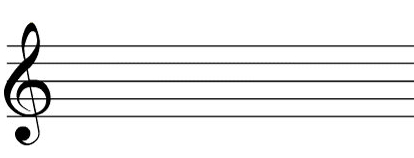
\includegraphics[width=0.8\textwidth]{./imagenes/pentagrama}
  \caption{Representación gráfica de un pentagrama} \label{fig:pentagrama}
  \end{figure}
\item Pulso: es el latido constante y regular de la música, siendo la unidad temporal básica y, en comparación con esta unidad de tiempo, se mide la duración de las notas y silencios.
\item “Tempo”: es la velocidad del pulso. Para indicar un tempo se utiliza como unidad los “bpm” (“Beats Per Minute”, es decir, los “Pulsos Por Minuto”). Así, si el tempo de una obra es de 60 bpm, tendremos que se producirá un pulso por segundo (1 bps) o lo que es lo mismo, cada un segundo, tendremos un pulso.
\item Ritmo: es la combinación de sonidos y silencios de diferente duración.
\item Compás: facilita la lectura de la música. En un pentagrama, los compases quedan divididos por líneas divisorias. Tomaremos que todos los compases son cuaternarios de subdivisión binaria (la mayoría de las obras para banda de música se encuentran compuestas para este tipo de compases o binarios -encajables en los anteriores- y así podremos simplificar el problema para su estudio aunque, como veremos durante la fase de implementación, esto es solo importante para entender mejor el diseño), es decir, un compás está dividido en cuatro notas negras (cada una será de un pulso de duración).
\end{itemize}

\section{Producto a desarrollar}

\paragraph{
Teniendo en cuenta todo lo dicho en las anteriores páginas, es el momento de manifestar qué dispositivo es el que se desea desarrollar en este trabajo: un sistema que marque el pulso (que no el ritmo, al poder ser éste irregular mientras que el pulso es constante) en función del “tempo” que indique el director de la agrupación. Además, el sistema deberá ser discreto ya que se busca que las bandas lo utilicen principalmente en la calle.
}

\paragraph{
Esta necesidad por parte de las bandas de música ha sido detectada por algunos fabricantes, como Peterson, que puso a la venta un producto llamado “Body Beat”. Dispone de un amplio abanico de funciones, pero su tamaño y su elevado coste hacen inviable la implantación del sistema en una banda de música (hay que tener en cuenta que el número de componentes en una banda es variable pero ronda entre los 50 y 100 músicos -algunas de ellas sobrepasan este número, como la “Banda de Cornetas y Tambores Nuestra Señora de la Victoria” conocida como “Las Cigarreras” de Sevilla \cite{cigarreras} que, en las fechas en las que se escribe este trabajo, ronda los 140 componentes-. Por otro lado, las dimensiones, de unos 10.8 cm x 7.6 cm x 2.54 cm puede que sean demasiado grandes). Como último escollo, muchos son los usuarios que, a través de la red, se quejan de la corta duración de la batería (teniendo en cuenta que hay actuaciones que pueden llegar a durar entre 8 y 10 horas, esto es un problema importante).
}

\paragraph{
Un dispositivo más barato con un número menor de funciones pero que permita la sincronización de todos los dispositivos y mantener el tempo durante toda la interpretación, atraería más usuarios. Si además se procura que la construcción se haga utilizando software y hardware libre, podría crearse una comunidad de desarrolladores en torno al producto, consiguiendo mejorar la calidad del dispositivo y aumentar la funcionalidad de este.
}

%
\chapter{Objetivos}
\title{Objetivos}
\title{Objetivos}

\paragraph{
Los principales objetivos a alcanzar con este desarrollo son:
}
  \begin{itemize}
    \item[\textbf{OBJ.1}] Que el sistema sea wireless: se quiere realizar un dispositivo que permita la comunicación con el resto de dispositivos del sistema sin necesidad de una conexión física entre ellos
    \item[\textbf{OBJ.2}] Conseguir un precio menor que otras soluciones del mercado: utilizando una tecnología distinta a la que han usado otros productos, tratar de obtener un sistema con un menor costo
    \item[\textbf{OBJ.3}] Escalable en el número de dispositivos: se quiere crear un sistema que disponga de una gran escalabilidad
    \item[\textbf{OBJ.4}] Ampliable en funciones: posibilidad de desarrollar nuevas funcionalidades partiendo de la funcionalidad más básica del sistema
    \item[\textbf{OBJ.5}] Vestible: debe ser un sistema discreto y cómodo para el portador
    \item[\textbf{OBJ.6}] Bajo consumo energético: se quiere desarrollar un sistema que no consuma demasiada energía para sacar el máximo partido a la batería que se inserte
    \item[\textbf{OBJ.7}] Tecnología lo más libre posible: se desea utilizar herramientas libres para tratar de atraer a desarrolladores para que colaboren en el proyecto. Además por la propia naturaleza del software/hardware libre, la comunidad aportará parches y soluciones a los problemas que puedan presentarse, mejorando la calidad del desarrollo
    \item[\textbf{OBJ.8}] Suficiente para cubrir las necesidades del mercado: aunque anteriormente se mencionaba que se desea que el sistema sea ampliable en funciones, es también necesario que la versión inicial tenga unas funciones mínimas que permitan cubrir las necesidades básicas del mercado
  \end{itemize}

\paragraph{
Como objetivos secundarios:
}
  \begin{itemize}
    \item[\textbf{obj.1}]Utilizar diversas versiones de la plataforma hardware Arduino: se tiene como objetivo utilizar distintas versiones de Arduino para poder obtener el producto con distintos formatos (Arduino Lilypad, Arduino Uno...)
    \item[\textbf{obj.2}]Desarrollar una red inalámbrica de sensores: teniendo en cuenta la actual dirección de la industria respecto a este tipo de tecnología (su aplicación, por ejemplo. en el “Internet de las Cosas” \cite{hypeIoT} \cite{gatnercurve}) , es interesante trabajar con esta tecnología
    \item[\textbf{obj.3}]Crear un dispositivo wearable: actualmente es uno de los sectores en los que más están trabajando las compañías. Si miramos la curva de Gatner \cite{gatnercurve}, en el año 2014 estas tecnologías se situaban en la cima del ciclo.
  \end{itemize}

%
\chapter{Especificación de Requisitos}
\label{cap:EspecificaciondeRequisitos}
\title{Especificación de Requisitos}

Para lograr que el desarrollo de un sistema hardware o software sea un éxito, es necesario que los desarrolladores comprendan totalmente las especificaciones que requiere el proyecto. En esta sección se va a proceder a enumerar los requisitos del sistema en el que se está trabajando.

\title{Modelado del sistema}
\section{
Modelado del sistema
}

El dispositivo que se desea desarrollar tiene que hacer la función básica
del director de la banda de música durante una actuación, es decir,
marcar el mismo pulso a los músicos.

Cuando la agrupación se encuentra realizando un concierto, el
esquema de comunicación que se sigue es el mostrado en la figura \ref{fig:modeladoconceptual}
(donde el nodo rojo es el director y lo morados los músicos). El único flujo de información
que hay es que que marcan las flechas (el pulso, que sigue un tempo constante). Hay que
aclarar que en este caso, para simplificar, sólo se han dibujado 5 músicos,
sin embargo, como se vio en la introducción, las bandas suelen contar entre sus filas con
varias decenas de integrantes.


\begin{figure}[htb]
\centering
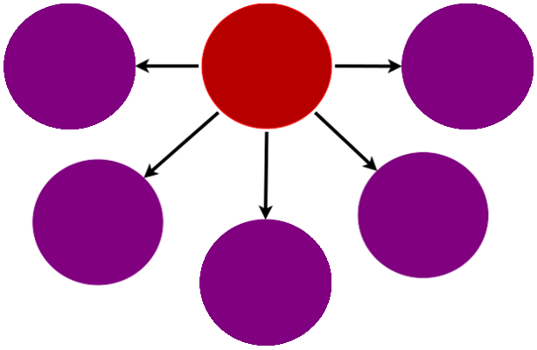
\includegraphics[width=0.6\textwidth]{./imagenes/modeladoconceptual}
\caption{Modelado del sistema} \label{fig:modeladoconceptual}
\end{figure}

El flujo de información es el mostrado en la figura \ref{fig:mensajesconceptual}

  \begin{figure}[htb]
  \centering
  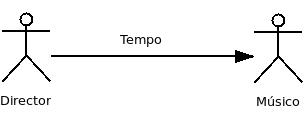
\includegraphics[width=0.6\textwidth]{./imagenes/mensajesconceptual}
  \caption{Traspaso de información} \label{fig:mensajesconceptual}
  \end{figure}


Es necesario guardar el ``tempo'' (que será establecido por el director) y algún tipo
de idenficación de los músicos, para que el director sepa con quién se tiene que
comunicar (aunque esto se verá más adelante).


\title{Actores}
\section{Actores}
\label{sec:actoresRequisitos}

Del esquema de la figura \ref{fig:mensajesconceptual} podemos sacar una conclusión clara:
será necesaria la distinción entre dos tipos de usuarios en nuestro sistema.

  \begin{itemize}
    \item Director: es el que envía el pulso al resto de actores. Solo uno por sistema
    \item Músico: recibe el pulso del director. Habrá multiples
  \end{itemize}


\title{Requisitos funcionales}
\section{Requisitos funcionales}

En este apartado se van a describir los requisitos funcionales del sistema.
Estos requisitos son aquellas funciones o capacidades que el sitema debe
tener para satisfacer las necesidades de los usuarios.

\begin{itemize}
    \item[\textbf{RF.1}] El sistema permitirá al director insertar un tempo
    \item[\textbf{RF.2}] Se capacitará al director para hacer llegar el pulso adecuado a los intérpretes
    \item[\textbf{RF.3}] El pulso se comunicará a los músicos a través de algún actuador (una señal visual, por ejemplo)
\end{itemize}


\title{Requisitos no funcionales}
\section{Requisitos no funcionales}

En estea sección se van a describir los distintos requisitos no funcionales del sistema.
Los requisitos no funcionales son aquellos que nos informan de restricciones que debe cumplir
nuestro sistema.


\begin{itemize}
    \item[\textbf{RNF.1}] El sistema debe ser wireless: la comunicación entre los
      dispositivos debe hacerse sin cables. Satisface el OBJ1
    \item[\textbf{RNF.2}] Debe de ser barato: para que el usuario desee utilizar
      el sistema, este debe tener un coste asumible. Satisface el OBJ2
    \item[\textbf{RNF.3}] La escalabilidad no debe ser un problema: se deben poder añadir
      muchos dispositivos al sistema y que la funcionalidad no se resienta. Satisface el
      OBJ3
    \item[\textbf{RNF.4}] Debe permitir que se puedan añadir funciones: para futuras mejoras.
      Satisface el OBJ4 y, en cierta forma, el OBJ7.
    \item[\textbf{RNF.5}] El dispositivo que se desarrolle tiene que ser discreto y cómodo:
      ningún usuario va a querer utilizarlo si se siente mal llevándolo o si es demasiado llamativo.
      Satisface el OBJ5
    \item[\textbf{RNF.6}] Bajo consumo energético: se busca aprovechar la batería al máximo
      (si el dispositivo funciona durante poco tiempo, no habrá usuarios que deseen utilizarlo).
      Satisface el OBJ6
    \item[\textbf{RNF.7}] Sincronización entre los músicos: ya que lo que se busca es dar unidad
      a la interpretación de las distintas obras, el sistema debe cumplir unos requisitos de tiempo
      importantes (a nivel de milisegundos para que, en caso de haber algo de asincronía, el usuario no lo note).
    \item[\textbf{RNF.8}] El pulso debe mantenerse constante: el pulso, por definición
      no cambia a lo largo de la obra y debe conseguirse que el usuario lo perciba de forma
      constante
\end{itemize}


\title{Requisitos de información}
\section{Requisitos de información}

Estos requisitos indican qué información guarda nuestro sistema.

  \begin{itemize}
    \item[\textbf{RI.1}] Tempo: se guardará el tempo indicado por el director
    para poder transmitir el pulso adecuado a los distintos músicos o, en su defecto,
    enviar el tempo una vez que estén sincronizados
    \item[\textbf{RI.2}] Músicos: el director deberá conocer los músicos existentes en la banda
    para saber a quién tiene que comunicarle el tempo. Podría darse el caso de dos
    agrupaciones musicales que se encontrasen muy próximas y utilizase en sistema:
    hay que evitar que el pulso de una de las bandas interfiera el de la otra
  \end{itemize}

%
\chapter{Planificación}
\title{Planificación}

\title{Metodología de desarrollo}
\section{Metodología de desarrollo}

\paragraph{
La metodología que se ha tratado de seguir para el desarrollo de este proyecto ha sido
un modelo en espiral ya que lo primero que se quiere solucionar es una funcionalidad
básica (mantener el mismo pulso entre todos los músicos). Sobre esto,
se desea que la comunidad (o los mismos desarrolladores), introduzcan nuevas
funcionalidades.
}

\paragraph{
Incluso dentro del desarrollo de la funcionalidad más básica (que es
la que se trata de implementar en este trabajo), se sigue el una metodología en espiral:
}

\begin{enumerate}
  \item Extracción de los requisitos
  \item Planificación
  \item Ingeniería
  \item Construcción
\end{enumerate}

\title{Fases}
\section{Fases}
\paragraph{
En la anterior sección se ha comentado la metodología a utilizar y, de forma general,
las fases a desarrollar. En esta sección se va a entrar en más detalle.
}

\begin{description}
  \item [Extracción de los requisitos]\hfill \\
  \begin{itemize}
    \item Descripción: obtención de los requisitos funcionales, no funcionales y de información del proyecto
    \item Apartado: Capítulo \ref{cap:EspecificaciondeRequisitos}
  \end{itemize}
  \item [Planificación]\hfill \\
    \begin{itemize}
      \item Descripción: estimación de costo, temporal, recursos humanos...
      \item Apartado: Este capítulo
    \end{itemize}
  \item [Ingeniería]\hfill \\
  \begin{itemize}
    \item Descripción: análisis de los requisitos y diseño del sistema a desarrollar
    \item Apartado: Capítulos \ref{cap:Analisis} y  \ref{cap:Diseno}
  \end{itemize}
  \item [Construcción]\hfill \\
  \item Descripción: implementación del proyecto
  \item Apartado: Capítulo \ref{cap:Implementacion}
\end{description}

\title{Estimación temporal}
\section{Estimación temporal}
\paragraph{
Teniendo en cuenta las partes detalladas en las sección anterior, es momento de
hacer una estimación temporal del proyecto.
}

\begin{itemize}
  \item Especificaciones del proyecto
  \begin{itemize}
    \item{Conocer adecuadamente las necesidades del usuario}
    \item{Establecer los objetivos del proyecto}
    \item{Extraer requisitos funcionales}
    \item{Extraer requisitos no funcionales}
    \item{Extraer requisitos de información}
    \item{Tiempo estimado: \textbf{15 horas}}
  \end{itemize}
\end{itemize}

\begin{itemize}
  \item Planificación
  \begin{itemize}
    \item{Calcular un presupuesto}
    \item{Establecer una temporización}
    \item{Establecer las fases}
    \item{Encontrar recursos que puedan ser reutilizables en el proyecto}
    \item{Definir los recursos humanos disponibles}
    \item{Tiempo estimado: \textbf{20 horas}}
  \end{itemize}
\end{itemize}

\begin{itemize}
  \item Análisis y diseño
  \begin{itemize}
    \item{Analizar los requisitos del proyecto}
    \item{Creación de diagramas}
    \item{Diseño de arquitectura}
    \item{Tiempo estimado: \textbf{40 horas}}
  \end{itemize}
\end{itemize}


\begin{itemize}
  \item Construcción
  \begin{itemize}
    \item{Establecer herramientas/plataformas/lenguaje/software a utilizar}
      \begin{itemize}
        \item{Decidir qué plataformas utilizar}
        \item{Investigar las herramientas de desarrollo de las plataformas}
        \item{Realizar pruebas para conocer si las plataformas son válidas para el proyecto}
      \end{itemize}
    \item{Comunicación entre los actores del sistema}
    \item{Cálculo de los valores necesarios para mantener el tempo en un actor}
    \item{Envío del tempo desde el director a los músicos}
    \item{Posibilidad de cambiar el tempo (por parte del director)}
    \item{Aplicaciones propias para cambiar el tempo}
    \item{Tiempo estimado: \textbf{100 horas}}
  \end{itemize}
\end{itemize}

\begin{itemize}
  \item Documentación
  \begin{itemize}
    \item{Documentar código}
    \item{Documentación del proyecto}
    \item{Creación de esquemas eléctricos para ayudar a futuros desarrolladores
    a comprender el conexionado}
    \item{Tiempo estimado: \textbf{40 horas}}
  \end{itemize}
\end{itemize}

\paragraph{
Se ha hecho una estimación de la cantidad de días que ocuparían todas
estas tareas y, para mostrarlo de una forma más gráfica,
se ha creado un diagrama de Grantt, que se puede ver en la figura \ref{fig:grantt}.
}

\begin{figure}[htb]
\centering
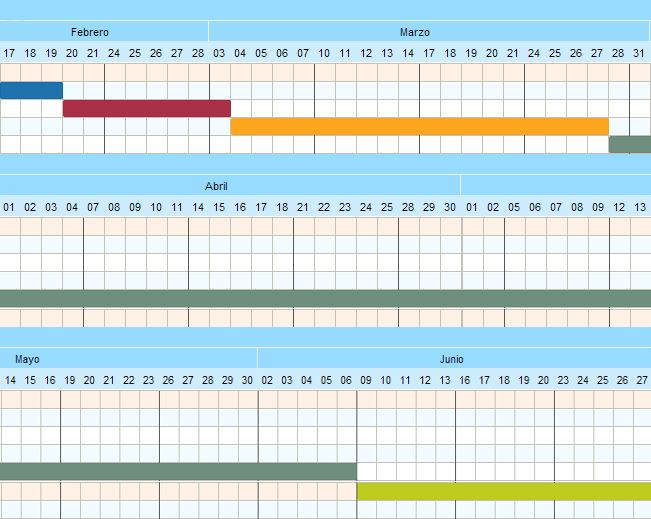
\includegraphics[width=1\textwidth]{./imagenes/grantt}
\caption{Diagrama de Grantt} \label{fig:grantt}
\end{figure}


\title{Recursos humanos}
\section{Recursos humanos}

\paragraph{
Gracias a que es un proyecto de software/hardware libre, todo aquel que
desee particiar en el proyecto puede hacerlo realizando aportaciones en los
\href{https://github.com/iblancasa/ArduBand}{repositorios del proyecto}.
}


\title{Recursos reutilizables}
\section{Recursos técnicos reutilizables}

\paragraph{
Estos recursos hacen referencia a anteriores desarrollos hardware o software creados
por otros desarrolladores o empresas.
}

\paragraph{
En el capítulo de implementación se explicará con más detalle por qué se
eligen los elementos que se van a describir en los dos siguientes apartados.
}


\subsection{Recursos software reutilizables}
\title{Recursos software reutilizable}


\paragraph{
En la introducción se hacía hincapié en la necesidad de crear una aplicación
Android para ayudar al director a establecer el tempo deseado. Por tanto,
serán recursos a tener en cuenta durante el desarrollo todas las herramientas
que implementa el propio SDK de Android y aquellas bibliotecas con licencia
libre que se encuentran en Internet (ya sean para añadir funcionalidad o elementos
gráficos).
}

\paragraph{
También se va a desarrollar un dispositivo físico que necesitará un software para estar
controlado. Todas las bibliotecas del controlador con licencia libre, también estarán
disponibles para su uso (en la sección de implementacion, veremos que se utilizará
Arduino -el cual tiene muchas bibliotecas disponibles- y XBee -existiendo para este
sistema de comunicación Wireless algunas bibliotecas desarrolladas por la comunidad-).
}


\subsection{Recursos hardware reutilizables}
\title{Recursos hardware reutilizable}

\paragraph{
Como se acaba de comentar, se utilizará la plataforma Arduino. Además de poder comprar
placas ya fabricadas, existe la posibilidad de crear una propia (es hardware libre y
los planos y software se encuentran disponibles en GitHub \cite{arduinoRepo}).
}

\paragraph{
Se utilizará también XBee, de la compañía Digi \cite{xbeedatasheet}.
}

\paragraph{
Por otro lado, se puede considerar el dispositivo móvil Android como un elemento a
tener en cuenta en esta sección (ya que es el elemento que hará de interfaz con el usuario,
eliminando la necesidad de crear un dispositivo físico para que el director interactúe con
el sistema).
}

\section{Presupuesto}
\title{Presupuesto}

\paragraph{En esta sección se va a proceder a estimar los costes del proyecto}.

\subsection{Licencias software y hardware}
\title{Licencias software y hardware}

\paragraph{
Gracias a la utilización de software y hardware libre, no es necesario el pago de licencias.
}

\paragraph{
El único problema que podría plantearse viene por parte de la empresa Digi al utilizar
el dispositivo XBee pero, debido a que este dispositivo está pensado para crear otros
nuevos, no existe problema en cuanto a su redistribución. X-CTU, el software que se va a
utilizar para la programación de los módulos no tiene licencia libre y se encuentra protegido
por derechos de autor, aunque se distribuye de manera gratuita \cite{licenciaXCTU}.
}

\subsection{Material}
\title{Material}

\paragraph{A continuación se listarán los materiales necesarios y su costo aproximado.}

  \begin{description}
    \item [Arduino]\hfill \\
      \begin{itemize}
        \item {Función: controlar los elementos hardware}
        \item {Precio aproximado: 7\euro}
      \end{itemize}
    \item [XBee]\hfill \\
      \begin{itemize}
        \item {Función: comunicación con el resto de dispositivos}
        \item {Precio aproximado: 25\euro}
      \end{itemize}
      \item [Bluetooth]\hfill \\
        \begin{itemize}
          \item {Función: comunicación entre el dispositivo ArduBand y un dispositivo móvil}
          \item {Precio aproximado: 6\euro}
        \end{itemize}
      \item [XBee Adapter/shield]\hfill \\
        \begin{itemize}
          \item {Función: permitir la conexión de XBee con Arduino}
          \item {Precio aproximado: 10\euro}
        \end{itemize}
      \item [Micromotor]\hfill \\
        \begin{itemize}
          \item {Función: actuador. Informa al músico del pulso}
          \item {Precio aproximado: 1.5\euro}
        \end{itemize}
      \item [Carcasa impresa]\hfill \\
          \begin{itemize}
            \item {Función: guardar los componentes de posibles golpes}
            \item {Precio aproximado: 1\euro}
        \end{itemize}
      \item [Varios]\hfill \\
        \begin{itemize}
          \item {Función: cableado, soldadura...}
          \item {Precio aproximado: 2\euro}
        \end{itemize}
  \end{description}

\paragraph{
Como Arduino es un proyecto de hardware libre, muchas empresas han decidido
dedicarse a crear sus propias placas compatibles con las originales pero a un
precio mucho menor. En este presupuesto se asume que se están utilizando estas
placas derivadas.
}

\paragraph{
A este material necesario se podría añadir las herramientas de las que se precisa
para el desarrollo.
}
\begin{description}
  \item [Teléfono Android]\hfill \\
    \begin{itemize}
      \item {Función: desarrollar y depurar la aplicación Android}
      \item {Precio aproximado: 150\euro}
    \end{itemize}
  \item [Dispositivo Android Wear]\hfill \\
    \begin{itemize}
      \item {Función: desarrollar y depurar la aplicación Android Wear}
      \item {Precio aproximado: 100\euro}
    \end{itemize}
\end{description}

\paragraph{En el caso del teléfono móvil se ha elegido (para el presupuesto) "Motorola Moto G" por tener
un precio basante ajustado y soportar la última versión de Android (cuando se escribe este
trabajo, la última versión es Android 5). Para dispositivo Android Wear (también para el presupuesto)
se ha elegido "LG G Watch" (por ser el dispositivo Android Wear más barato del momento
y que, con las funcionalidades de las que dispone, permite llevar a cabo el desarrollo).}

\subsection{Recursos humanos}
\title{Recursos humanos}


\subsection{Otros gastos}
\title{Otros gastos}
\paragraph{
Teniendo en cuenta que se va a desarrollar una aplicación Android y otra Android Wear,
será necesario pagar la cuota para obtener licencia de desarrollo (25USD, unos 22.5\euro) \cite{desarrollaAndroid}.
}

%
\chapter{Análisis}
\title{Análisis}
\label{cap:Analisis}

\paragraph{
En este capítulo se analizarán los requisitos del proyecto para, más tarde, poder
realizar el diseño.
}

\title{Actores}
\section{Actores}
\paragraph{
Ya en la sección \ref{sec:actoresRequisitos} se hizo alusión a la existencia de
dos tipos de actores. Ahora se profundizará un poco más en su análisis.
}

\begin{itemize}
  \item \textbf{Ac-1.} Director
  \begin{itemize}
   \item Descripción: es quien decide el tempo que debe seguir la banda y comunicar el pulso
   a los músicos
   \item Características: solo hay uno
   \item Relaciones: conocerá a todos los músicos
   \item Atributos: ninguno
   \item Comentarios: tiene la responsabilidad del correcto funcionamiento del sistema
  \end{itemize}

  \item \textbf{Ac-1.} Músico
  \begin{itemize}
     \item Descripción: recibe el pulso del director
     \item Características: hay muchos
     \item Relaciones: conocerá al director. No necesita conocer al resto de músicos
     \item Atributos: ninguno
     \item Comentarios: recibirá el pulso enviado por el director con algún tipo de actuador
  \end{itemize}
\end{itemize}

\title{Casos de uso}
\section{Casos de uso}


\begin{table}[!htbp]
\centering
\label{CU1}
\begin{tabular}{|
>{\columncolor[HTML]{CBCEFB}}l |l|l|}
\hline
{\bf Caso de uso}   & Encender sistema                                    & {\it CU.1}                             \\ \hline
{\bf Actores}       & \multicolumn{2}{l|}{Director}                                                                \\ \hline
{\bf Tipo}          & \multicolumn{2}{l|}{Primario, esencial}                                                      \\ \hline
{\bf Precondición}  & \multicolumn{2}{l|}{}                                                                        \\ \hline
{\bf Postcondición} & \multicolumn{2}{l|}{El sistema quedará listo para usarse}                                    \\ \hline
{\bf Propósito}     & \multicolumn{2}{l|}{Iniciar el sistema}                                                      \\ \hline
{\bf Resumen}       & \multicolumn{2}{l|}{\begin{tabular}[c]{@{}l@{}}El sistema deberá guardar el
  tempo indicado por el \\ director de la banda\end{tabular}} \\ \hline
{\bf Autor}         & Israel Blancas Álvarez                              & Versión 1.0                            \\ \hline
\end{tabular}
\end{table}

\begin{table}[!htbp]
\centering
\label{CU2}
\begin{tabular}{|
>{\columncolor[HTML]{CBCEFB}}l |l|l|}
\hline
{\bf Caso de uso}   & Insertar tempo                                                          & {\it CU.2}                                                 \\ \hline
{\bf Actores}       & \multicolumn{2}{l|}{Director}                                                                                                        \\ \hline
{\bf Tipo}          & \multicolumn{2}{l|}{Primario, esencial}                                                                                              \\ \hline
{\bf Precondición}  & \multicolumn{2}{l|}{El sistema debe haberse encendido}                                                                               \\ \hline
{\bf Postcondición} & \multicolumn{2}{l|}{El sistema guardará el tempo}                                                                                    \\ \hline
{\bf Propósito}     & \multicolumn{2}{l|}{Guardar tempo}                                                                                                   \\ \hline
{\bf Resumen}       & \multicolumn{2}{l|}{\begin{tabular}[c]{@{}l@{}} El pulso es enviado desde el director a los músicos. \\
De esta forma quedarán sincronizados y conociendo \\ el tempo \end{tabular}} \\ \hline
{\bf Autor}         & Israel Blancas Álvarez                                                  & Versión 1.0                                                \\ \hline
\end{tabular}
\end{table}

\begin{table}[!htbp]
\centering
\label{CU3}
\begin{tabular}{|
>{\columncolor[HTML]{CBCEFB}}l |l|l|}
\hline
{\bf Caso de uso}   & Enviar pulso                           & {\it CU.3}                \\ \hline
{\bf Actores}       & \multicolumn{2}{l|}{Director, Músico}                              \\ \hline
{\bf Tipo}          & \multicolumn{2}{l|}{Primario, esencial}                            \\ \hline
{\bf Precondición}  & \multicolumn{2}{l|}{Debe haberse insertado un tempo en el sistema} \\ \hline
{\bf Postcondición} & \multicolumn{2}{l|}{El pulso será comunicado a los músicos}        \\ \hline
{\bf Propósito}     & \multicolumn{2}{l|}{Enviar pulso desde el director a los músicos}  \\ \hline
{\bf Resumen}       & \multicolumn{2}{l|}{}                                              \\ \hline
{\bf Autor}         & Israel Blancas Álvarez                 & Versión 1.0               \\ \hline
\end{tabular}
\end{table}

\begin{table}[!htbp]
\label{CU4}
\begin{tabular}{|
>{\columncolor[HTML]{CBCEFB}}l |l|l|}
\hline
{\bf Caso de uso}   & Atender al tempo                                 & {\it CU.4}                         \\ \hline
{\bf Actores}       & \multicolumn{2}{l|}{Músico}                                                           \\ \hline
{\bf Tipo}          & \multicolumn{2}{l|}{Primario, esencial}                                               \\ \hline
{\bf Precondición}  & \multicolumn{2}{l|}{El Director debe estar transmitiendo el pulso}                    \\ \hline
{\bf Postcondición} & \multicolumn{2}{l|}{El Músico conocerá el pulso y quedará sincronizado}               \\ \hline
{\bf Propósito}     & \multicolumn{2}{l|}{Sincronizar al sistema}                                           \\ \hline
{\bf Resumen}       & \multicolumn{2}{l|}{El director encenderá el sistema y todo se podrá poner en marcha} \\ \hline
{\bf Autor}         & Israel Blancas Álvarez                           & Versión 1.0                        \\ \hline
\end{tabular}
\end{table}

%
\chapter{Diseño}
\title{Diseño}
\label{cap:Diseno}

\section{Arquitectura}
Como se ha ido viendo en los capítulos anteriores, el dispositivo que se desea desarrollar
tiene que hacer la función básica del director de la banda de música durante una actuación,
es decir, marcar el mismo pulso a los músicos.
Si recordamos el esquema planteado en la figura \ref{fig:modeladoconceptual} y todo lo
que se ha ido desarrollando a través de los capítulos anteriores, podemos decir
que el sistema sigue una arquitectura de repositorio -o pizarra- (siendo el repositorio activo):

\begin{itemize}
  \item El director es el centro de todo. Se encarga de realizar la comunicación con los músicos
  \item Los músicos son subsistemas independientes (aunque tengan que estar sincronizados)
  \item Alto acoplamiento entre los músicos y el director
\end{itemize}

A parte de la relación existente entre músicos y director, no debemos olvidar que
deseamos comunicarnos desde un dispositivo (Android según las especificaciones pero que,
como se verá en la implementación, valdrá cualquier SO). Es por ello que el diagrama
de despliegue queda como en la figura \ref{fig:diagramadespliegue}.


\begin{figure}[htb]
\centering
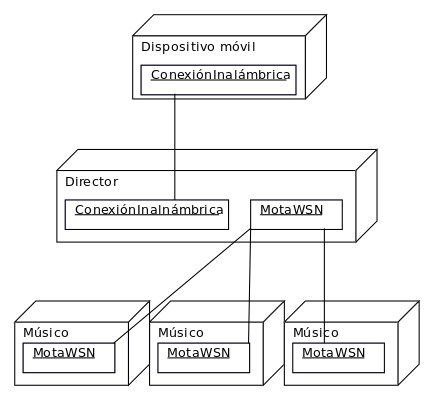
\includegraphics[width=1\textwidth]{./imagenes/diagramadespliegue}
\caption{Diagrama de despliegue} \label{fig:diagramadespliegue}
\end{figure}

\section{Diagramas de comunicación}
\title{Diagramas de comunicación}

Los casos de uso expuestos en \ref{subsec:casosdeuso} se han sideñado según
se muestra en las figuras \ref{fig:comunicacion1},  \ref{fig:comunicacion2} y
\ref{fig:comunicacion3}.


\begin{figure}[htb]
\centering
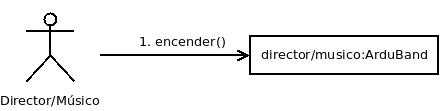
\includegraphics[width=1\textwidth]{./imagenes/comunicacion1}
\caption{Diagrama de comunicación 1} \label{fig:comunicacion1}
\end{figure}

\begin{figure}[htb]
\centering
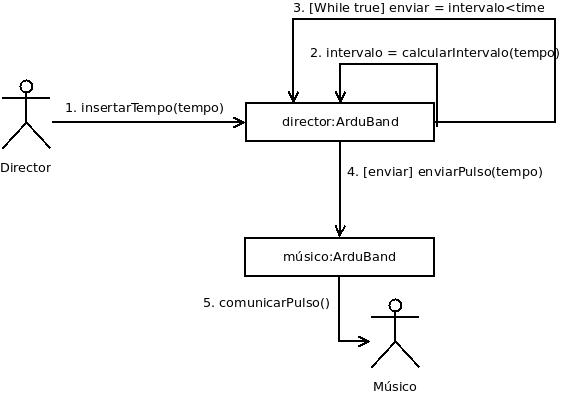
\includegraphics[width=1\textwidth]{./imagenes/comunicacion2}
\caption{Diagrama de comunicación 2} \label{fig:comunicacion2}
\end{figure}


\begin{figure}[htb]
\centering
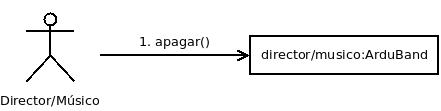
\includegraphics[width=1\textwidth]{./imagenes/comunicacion3}
\caption{Diagrama de comunicación 3} \label{fig:comunicacion3}
\end{figure}

%
\chapter{Implementación}
\title{Implementación}
\label{cap:Implementacion}


\section{Red}
\title{Red}

En el sistema a desarrollar, ya se ha manifestado la intención de crear distintos
tipos de dispositivos. También es necesario establecer una comunicación entre ellos,
es decir, una red. A lo largo de las siguientes secciones iremos viendo cómo se
ha implementado.\\

\subsection{Topología}
\title{Topología}
En primer lugar hay que remitirse a los distintos diagramas que se han ido
realizando para explicar la estructura propuesta, como el diagrama de despliegue (figura \ref{fig:diagramadespliegue}).\\

Se observa que todos los nodos (músicos) se comunican, única y exclusivamente, con un nodo central (director).
Es por elo que la topología de nuestra red debe ser una \textbf{topología en estrella}.\\

\subsection{Red inalámbrica de sensores}
\title{Red inalámbrica de sensores}

Para crear la red se va a optar por formar una red inalámbrica de sensores ya que es
el tipo de infraestructura que cumple con las necesidades del sistema a desarrollar.\\

Una red inalámbrica de sensores (\textit{WSN, Wireless Sensor Network}) es aquella formada por un
conjunto de elementos autónomos cuyo objetivo es el de solucionar una tarea utilizando
comunicación inalámbrica. Los nodos que forman la red no disponen de alta capacidad funcional
y tienen un costo energético bajo (siendo posible su alimentación a través de baterías de poca capacidad).\\

\begin{figure}[htb]
\centering
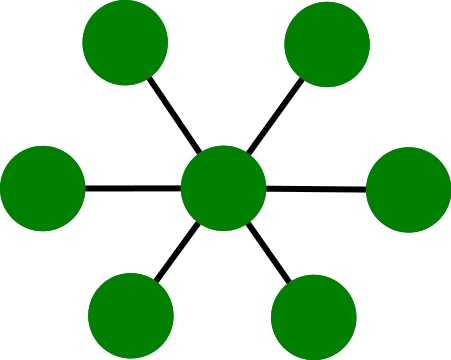
\includegraphics[width=0.6\textwidth]{./imagenes/estrella}
\caption{Topología en estrella} \label{fig:estrella}
\end{figure}

\subsection{Método a utilizar}
\title{Método a utilizar}
Dentro de las \textit{WSN}, podemos elegir entre distintos métodos para realizar la
comunicación entre nuestras motas. Según las necesidades que tenga nuestra red,
utilizaremos uno u otro. Se van a analizar brevemente algunos de los principales:

\begin{description}
  \item[WiFi] \hfill \\
    Basado en el estándar IEEE 802.11. Alta velocidad en transferencia de datos
    (permite adaptación a la velocidad de transmisión) y seguridad en la red pero
    no dispone de mecanismos para ahorrar energía
  \item[Bluetooth] \hfill \\
    Otro estándar de comunicación entre dispositivos. Permite broadcast, una velocidad
    de hasta 24Mbit/s y sus redes son de hasta 8 nodos (uno maestro y siete esclavos).
    En la versión 4 se han introducido métodos para reducir el consumo de energía
  \item[802.15.4] \hfill \\
    Es un estándar propuesto por el IEEE. El ancho de banda es muy pequeño, la latencia
    se sitúa en torno a los 15ms, alcance de entre 10 y 20 metros, permite tener miles
    de nodos en la red, mecanismos para tener un bajísimo consumo de energía y barato
  \item[ZigBee] \hfill \\
    Es un estándar desarrollado sobre 802.15.4, lo que quiere decir que añade capas a la
    propuesta hecha en 802.15.4 (añadiendo algunas funciones)
\end{description}

Todos estos métodos permiten la topología en estrella.\\

Teniendo en cuenta el análisis anterior se concluye que:
\begin{itemize}
  \item WiFi queda descartado: aunque existan redes de sensores que utilicen esta tecnología,
  WiFi no contempla mecanismos para el ahorro de energía. Aunque vaya a ser necesaria una alta velocidad
  (debido a los requisitos temporales del sistema), no hace falta tanta como la que
  proporciona este mecanismo de comunicación (por lo que se vería desperdiciada)
  \item Bluetooth se descarta: a través de la capa de aplicación, algunas implementaciones
  de redes inalámbricas de sensores han conseguido aumentar el número máximo de nodos por red.
  Por otra parte, aunque la versión 4 de Bluetooth esté pensada para economizar el gasto energético,
  este sigue siendo demasiado alto (es algo que cualquier usuario experimenta día a día cuando
  conecta unos auriculares, un manos libres o una smartband a su smartphone, descendiendo el nivel de
  carga de la batería a una velocidad muy alta)
  \item 802.15.4 o ZigBee son la solución: cumplen con casi todos los requisitos.
  El problema que puede presentarse viene dado por las velocidades de transferencia: aunque no
  se necesite realizar grandes traspasos de información, las comunicaciones deben
  hacerse de la manera más rápida posible. Hay que tener en cuenta que ZigBee está construido a partir
  de 802.15.4, lo que significa que la latencia será mayor (habrá que sumar la de 802.15.4 a la que provoquen
  las capas que añade ZigBee). También puede ocurrir que en el canal en el que se estén realizando las comunicaciones
  se esté produciendo otra (en ese caso, la velocidad de transmisión disminuirá)
\end{itemize}

\begin{figure}[htb]
\centering
\captionsetup{justification=centering}
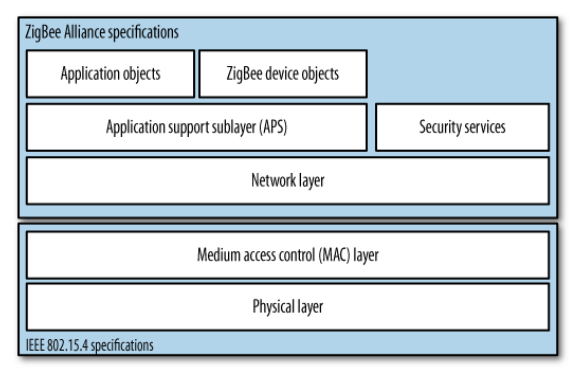
\includegraphics[width=1\textwidth]{./imagenes/zigbeestack}
\caption{ZigBee Stack \\
\scriptsize{Imagen extraída de \cite{faludi} (figura 8.1)} } \label{fig:stackzigbee}
\end{figure}

Finalmente se ha elegido trabajar con ZigBee aunque, probablemente, con 802.15.4 sería suficiente (incluso
mejor al tener una menor latencia). El motivo de esta selección viene determinado porque las motas disponibles
en el laboratorio son de tipo ZigBee, no habiendo de la otra variedad.\\

Para ser más específicos, se va a utilizar el modelo ``XBee 2mW Wire Antenna - Series 2 (ZigBee Mesh)", cuya referencia es
``XB24-Z7WIT-004" (ID: OUR XBEE2 e IC: 4214A-XBEE2) y que es la implementación de la compañía ``Digi" \cite{productdetaildigi}.


\begin{figure}[htb]
\centering
\captionsetup{justification=centering}
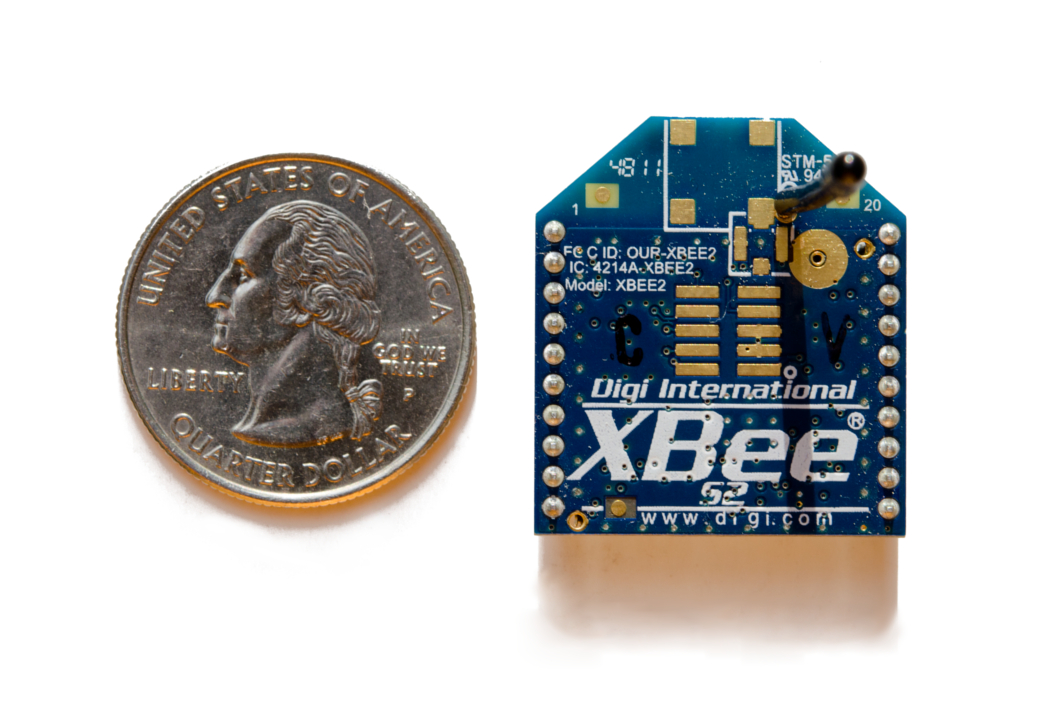
\includegraphics[width=1\textwidth]{./imagenes/xbeequarter}
\caption{Una mota XBee junto a un cuarto de dólar\\
\scriptsize{Imagen extraída de https://en.wikipedia.org/wiki/XBee} } \label{fig:xbeequarter}
\end{figure}

\begin{figure}[htb]
\centering
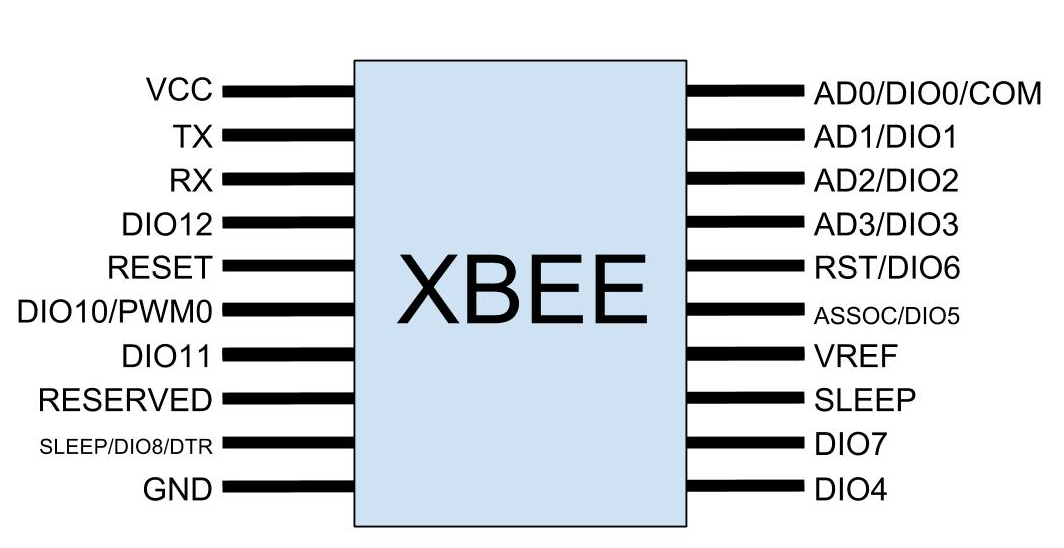
\includegraphics[width=1\textwidth]{./imagenes/xbeepinout}
\caption{XBee PINOUT} \label{fig:xbeepinout}
\end{figure}

En la figura \ref{fig:xbeepinout} podemos ver el esquema de XBee Series 2.

\begin{itemize}
  \item VCC: alimentación
  \item TX: pin de salida de comunicación serial
  \item RX: pin de entrada de comunicación serial
  \item DIO12: entrada o salida digital
  \item Reset: permite resetear el módulo
  \item DIO10/PWM0/RSSI: tiene tres funcionalidades (entrada/salida digital,
    RSSI -”Indicador de Intensidad de la Señal”- o pin de modulación por ancho de pulsos)
  \item DIO11: entrada o salida digital
  \item Reserved: es un pin reservado. No se aconseja conectarlo a nada
  \item SLEEP/DIO8/DTR: también dispone de varias funciones (control de sueño de la mota,
    entrada/salida o señal hardware de handshaking).
  \item GND: tierra
  \item DIO4: entrada o salida digital
  \item DIO7: entrada o salida digital. También puede hacer las funciones de “clear to send”
  \item SLEEP: indicador de sueño. Permite saber si la mota se encuentra durmiendo
    o no (si el estado es alto, se encuentra en funcionamiento)
  \item VFREF: no tiene funcionalidad en este modelo
  \item ASSOC/DIO5: doble función (indicador de pertenencia a red -estado alto si
    está asociada a una red- o entrada/salida digital)
  \item RST/DIO6: doble función (petición de envío o entrada/salida digital)
  \item AD3/DIO3: entrada salida analógica o digital
  \item AD2/DIO2: entrada salida analógica o digital
  \item AD1/DIO1: entrada salida analógica o digital
  \item AD0/DIO0/COM: triple funcionalidad (entrada/salida digital o analógica o puesta en servicio)
\end{itemize}

Sus características técnicas (que se pueden consultar en \cite{xbeedatasheet}) son:
\begin{itemize}
  \item 3.3V @ 40mA
  \item Velocidad máxima: 250kbps
  \item 2mW salida (+3dBm)
  \item 400ft (120m) rango
  \item Antena incorporada
  \item Certificado por FCC
  \item 6 10-bit ADC pines de entrada
  \item 8 pines digitales de entrada/salida
  \item 128-bit encriptación
  \item Modo AT o API
\end{itemize}

En este último punto se nos hablan de dos modos de funcionamiento:

\begin{description}
  \item[AT] \hfill \\
    Es el modo transparente. Una vez establecida la configuración (mediante comandos
    que se envían al dispositivo a través de serial), el dispositivo solo es capaz de
    comunicarse con la mota cuya dirección MAC corresponde con la de la configuración
    (también pueden enviarse paquetes a todos los dispositivos en caso que la dirección
    que se haya configurado sea la de broadcast). Esto quiere decir que, en caso que
    deseemos cambiar el destino de nuestras comunicaciones, tendremos que reconfigurar
    la mota (ya sea enviando comandos AT o utilizando algún software que los envíe
    por nosotros) Es el modo más simple de trabajar con XBee.
 \item[API] \hfill \\
    Este modo permite mucho más. Capacita al desarrollador a:
      \begin{itemize}
        \item Obtener RSSI (fortaleza de la señal respecto a otro dispositivo),
        \item Enviar paquetes a múltiples destinos
        \item Recibir paquetes de distintos tipos
        \item Activar funciones de integridad de datos, recibir ACK...
        \item Conocer el estado de la red
      \end{itemize}
\end{description}



\subsection{Modo API}
\title{Modo API}

Mientras que en el modo transparente los caracteres que escribamos en el puerto
serial de XBee serán enviados directamente a la mota destino, en este modo las
comunicaciones se realizan enviando paquetes con una estructura predefinida.\\

Existen dos formas de comunicarse con la mota cuando se encuentra en este modo:
\begin{itemize}
  \item Pines de entrada/salida: en el caso de querer dar una salida, la deberemos preestablecer en la configuración.
  Un pin que se configure en modo entrada, tomará el valor que le llegue y la mota enviará el valor a la mota destino.
  La propia mota genera el paquete y lo envía.
  \item Puerto serial: permite la creación y envío de distintos tipos de paquetes.
  Esto se hace de forma manual, es decir, se precisa de un controlador que escriba los valores en el puerto serial de XBee.
\end{itemize}

Cada paquete que envía (o recibe) un dispositivo XBee, tiene la estructura de la figura \ref{fig:tramaapi}.

\begin{figure}[htb]
\centering
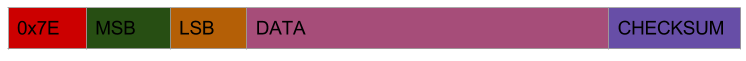
\includegraphics[width=1\textwidth]{./imagenes/tramaapi}
\caption{Paquete XBee en modo API} \label{fig:tramaapi}
\end{figure}

\begin{itemize}
  \item 0x7E: comienzo de la trama
  \item MSB: byte más significativo para la traza
  \item LSB: byte menos significativo para la traza
  \item DATA: puede incluir varias cosas, como el tipo de comando API o AT que se está enviando, parámetros… (para conocer más, )
  \item CHECKSUM: checksum de la trama
\end{itemize}

Para generar estas tramas utilizaremos una biblioteca open source que se encuentra en GitHub (\cite{libraryArduinoXBee}).
Gracias a ella, no tendremos que preocuparnos de generar los distintos elementos del paquete
(como el delimitador de comienzo o el cálculo del checksum).\\

Para conocer más sobre el modo API, el lector puede consultar el capítulo 5 (\textit{API and a Sensor Network}) de \cite{faludi}.\\

\subsection{XCTU: el software para manipular las motas}
\title{XCTU: el software para manipular las motas}
Este software es distribuido gratuitamente por Digi \cite{licenciaXCTU} y se puede descargar desde la página oficial
de dicha empresa.

Para conectar XBee a nuestro ordenador, debemos conectar las patillas de XBee del puerto serial a un
FTDI (por ejemplo) y con una conexión serial o USB, a nuestro ordenador. Otra posibilidad es obtener
una placa ``XBee Explorer" como la de la figura \ref{fig:xbeeexplorer}.


\begin{figure}[htb]
\centering
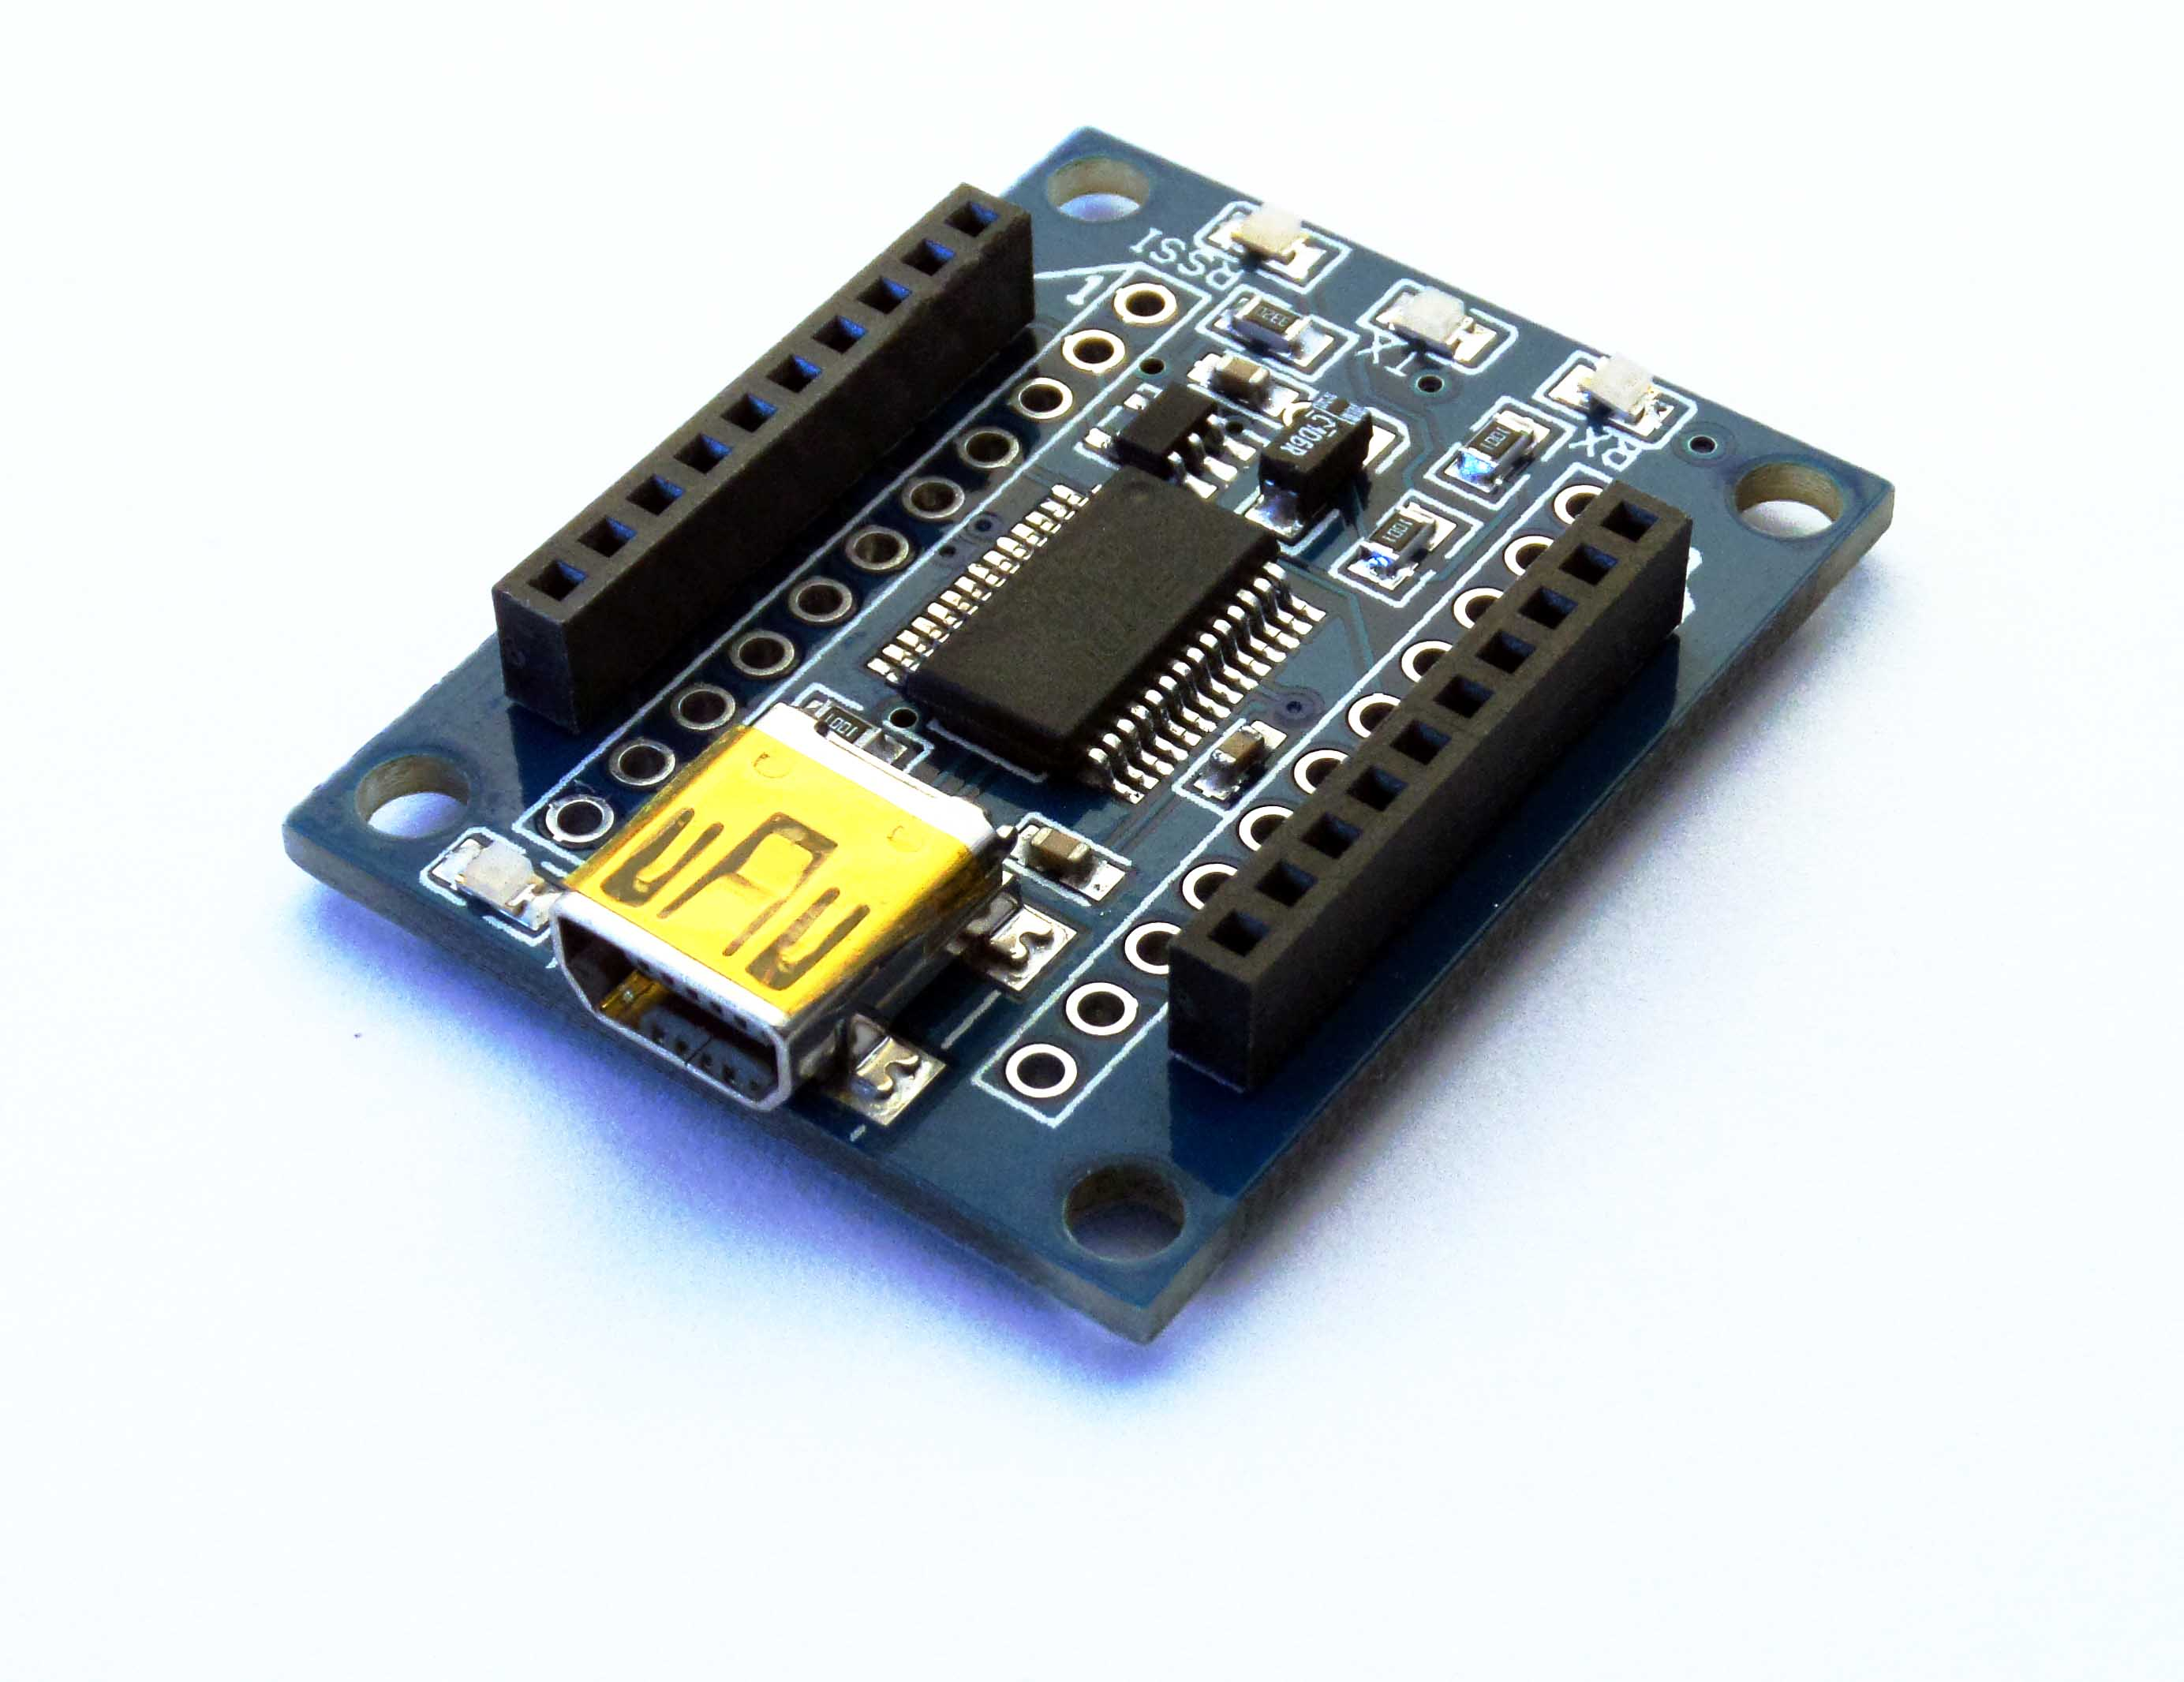
\includegraphics[width=0.8\textwidth]{./imagenes/xbeeexplorer}
\caption{XBee USB Explorer. Imagen extraída de \scriptsize{http://xbee.cl/xbee-explorer-usb/}} \label{fig:xbeeexplorer}
\end{figure}


En la ventana principal tenemos tres secciones: a la izquierda, la lista de los dispositivos
que tenemos conectados a nuestro ordenador; a la derecha, un panel de administración que variará
en función de lo que estemos haciendo con la mota; y arriba, las opciones relacionadas con el descubrimiento
de nuevos dispositivos (izquierda) o distintas acciones sobre la mota (derecha). Podemos verlo en la figura \ref{fig:interfaz1}.\\

\begin{figure}[!htb]
\centering
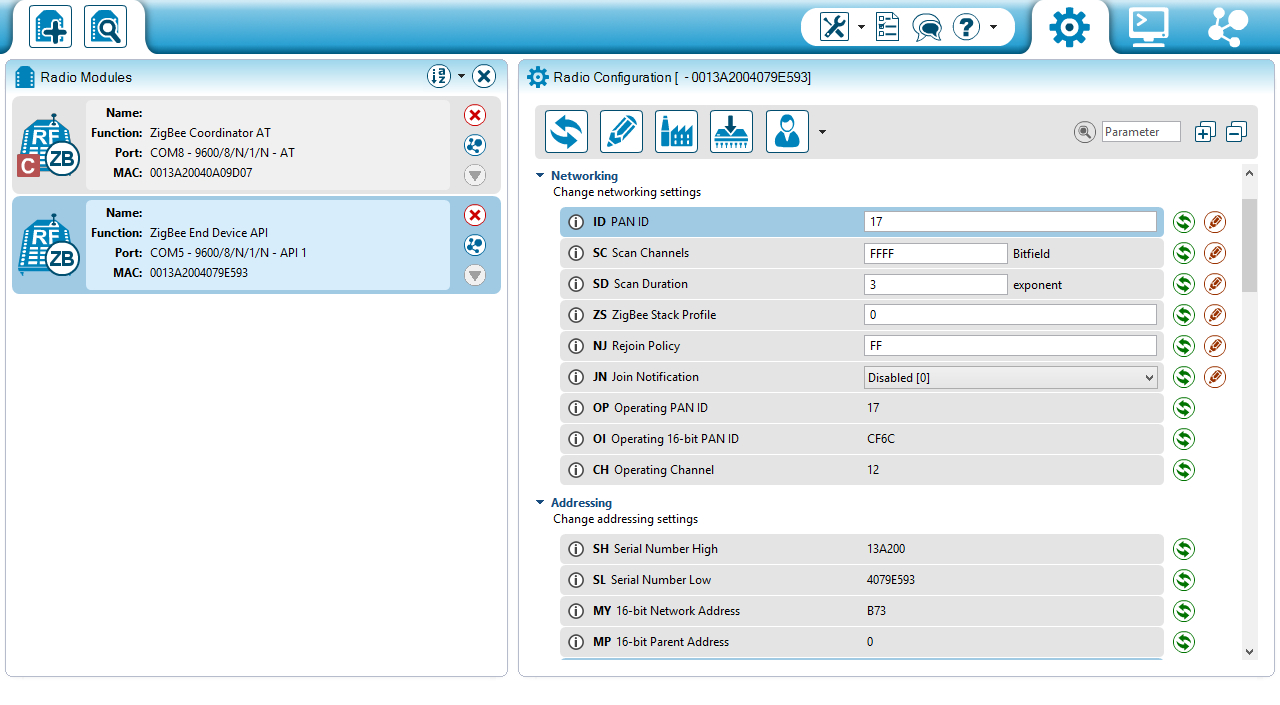
\includegraphics[width=1\textwidth]{./imagenes/interfaz1}
\caption{Interfaz XCTU} \label{fig:interfaz1}
\end{figure}

Lo primero que tendremos que hacer una vez hayamos conectado nuestra mota al ordenador, será descubrirla con XCTU
utilizando una de las dos opciones que tenemos arriba a la izquierda (es importante mencionar que, en caso que se nos
pida resetear la mota y, como es el caso de nuestro modelo, no tengamos un botón para resetear, deberemos unir con un
cable la patilla \guillemotleft RST\guillemotright con \guillemotleft GND\guillemotright).\\

\begin{figure}[!htb]
\centering
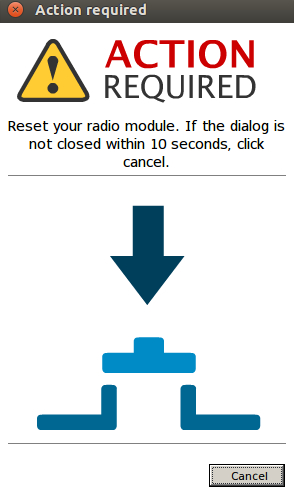
\includegraphics[width=0.5\textwidth]{./imagenes/xctureset}
\caption{Paquete XBee en modo API} \label{fig:xctureset}
\end{figure}

Una vez que tengamos la mota descubierta tendremos el menú de configuración (el de la rueda dentada) abierto. En él podremos
cambiar el firmware, volver a los ajustes de fábrica, establecer un nombre para la mota, ver la dirección de destino,
\textit{PAN} (Personal Area Network) a la que unirse... en función del firmware que tenga instalado la mota, habrá unas opciones u otras
(por ejemplo, en caso de tener un dispositivo final, podremos configurar cada cuánto tiempo de inactividad puede el nodo
entrar en suspensión).\\

En el siguiente menú, podremos ver qué es lo que está recibiendo (o enviando) nuestro XBee.
Se monitoriza el puerto serial (ver figura \ref{fig:interfaz2}).\\

\begin{figure}[!htb]
\centering
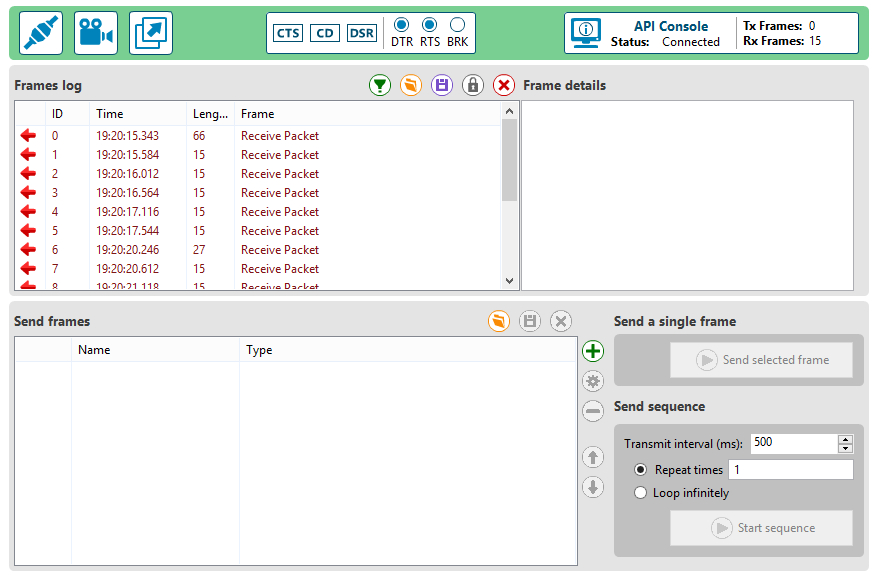
\includegraphics[width=1\textwidth]{./imagenes/interfaz2}
\caption{Monitorizando el puerto serial (modo API) en XCTU} \label{fig:interfaz2}
\end{figure}

Finalmente el tercer menú nos brinda algunas opciones relacionadas con la nube de Digi y la posibilidad
de conocer qué nodos están interconectados en la red (solo disponible si el módulo está en modo API).\\

\subsection{Posible problema de escalabilidad}
\title{Posible problema de escalabilidad}

Aunque estas redes están pensadas para contar con miles de dispositivos,
estas suelen estar formadas por un coordinador y varios routers.
Al haber solamente un coordinador, es éste quien debe almacenar
toda la información que concierne a la red.\\

La dirección MAC de una mota se divide en dos partes iguales (dirección alta y dirección baja).
Teniendo en cuenta que la MAC tiene un tamaño de 64 bits, cada parte tiene un total de 32 bits.
La dirección alta es la misma para todos los nodos y la baja es la que cambia. Por tanto, tendremos 2\textsuperscript{32} direcciones
disponibles (más de 4.000.000.000) o lo que es lo mismo, podremos direccionar hasta 2\textsuperscript{32} dispositivos.\\

El problema que se presenta es el siguiente: Cada dirección ocupa 64 bits, osea, 8 bytes. Si deseamos guardar 150
direcciones (en la introducción se hablaba de casos en los que había bandas que superan los 100 integrantes por lo que
deberíamos pensar en guardar un número mayor de direcciones, donde cada dirección sería un músico), tendremos que almacenar
1.200 bytes (8 bytes x 150 direcciones), unos 1.17KB. Si la memoria destinada a direcciones en la mota es menor que este tamaño,
pueden producirse problemas.\\

Ya que no se disponen de tantos dispositivos para hacer un experimento ni se ha encontrado información al respecto,
no podemos predecir el comportamiento del sistema ante tal número de nodos.\\

\section{Controlador}
\title{Controlador}

Para llevar a cabo el control de los componentes es necesario algún tipo de microcontrolador
o placa controladora. Se han estudiado dos posibles soluciones:

\begin{description}
  \item[PIC] \hfill \\
    \begin{itemize}
      \item Son microcontroladores
      \item Precio muy bajo
      \item Gran variedad
      \item Pequeño tamaño
      \item Programación en ensamblador, con una media de 35 instrucciones
      \item Simples pero orientados a un público muy relacionado con la programación
    \end{itemize}
    \begin{figure}[!htb]
    \centering
    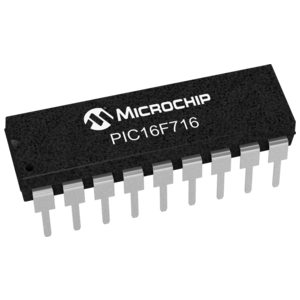
\includegraphics[width=0.5\textwidth]{./imagenes/pic}
    \caption{PIC16F716\\  \scriptsize{Imagen extraída de http://www.microchip.com/}} \label{fig:pic}
    \end{figure}
  \item[Arduino] \hfill \\
    \begin{itemize}
      \item Placa con un microcontrolador
      \item Programación en alto nivel (Python, Scratch, JavaScript o un derivado de Processing)
      \item Muchas bibliotecas para extender funcionalidad
      \item Existe una versión Wear (Arduino Lilypad, mostrado en la figura \ref{fig:lilypad})
      \item Shields para XBee (como la que se muestra en la figura \ref{fig:lilypadxbee})
    \end{itemize}
    \begin{figure}[!htb]
    \centering
    \captionsetup{justification=centering}
    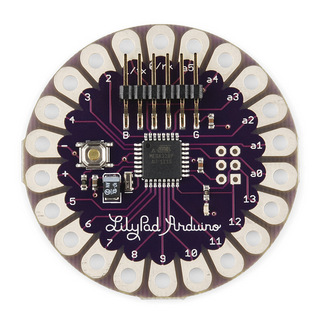
\includegraphics[width=0.5\textwidth]{./imagenes/lilypad}
    \caption{Arduino Lilypad\\
     \scriptsize{Imagen extraída de https://www.arduino.cc}} \label{fig:lilypad}
    \end{figure}

    \begin{figure}[htb]
    \centering
    \captionsetup{justification=centering}
    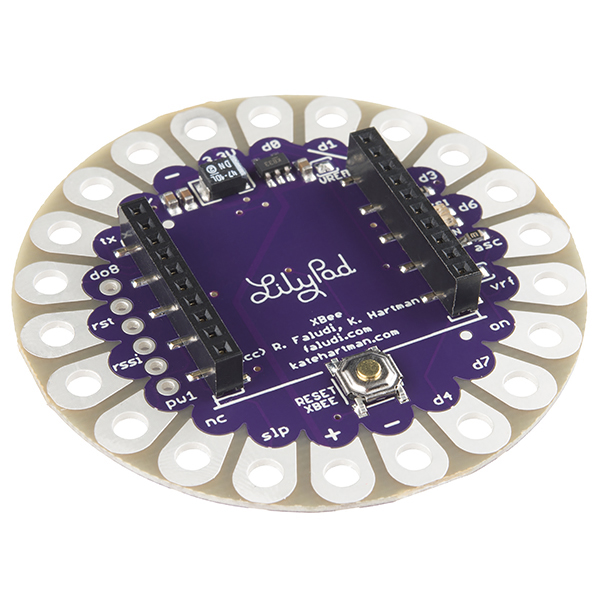
\includegraphics[width=0.5\textwidth]{./imagenes/lilypadxbee}
    \caption{Shield XBee Lilypad\\
      \scriptsize{Imagen extraída de https://www.faludi.com/ \cite{faludi}}} \label{fig:lilypadxbee}
    \end{figure}
\end{description}


\clearpage

Sabiendo que Arduino se encuentra orientado a un público con una menor formación en electrónica y
programación (por lo tanto, accesible a una mayor comunidad), se adecua más al objetivo de este proyecto.
También hay que tener en cuenta la cantidad de bibliotecas
existentes en Arduino (lo que nos ayudará a abstraernos de algunas tareas). Por contra,
PIC es más competitivo en tamaño y precio.\\

\subsection{IDE Arduino}
\title{IDE Arduino}

El IDE de Arduino puede ser descargado de su página oficial \cite{arduinoWeb}. Es de código abierto y se
encuentra basado, igual que el lenguaje que se utiliza, en Processing (un lenguaje basado a su vez en Java y C).

En el menú superior tenemos acceso a distintas opciones como guardar nuestro proyecto, cargar un proyecto de ejemplo,
instalar nuevas bibliotecas, seleccionar la placa para la que estamos desarrollando, el puerto en el que se encuentra dicha
placa...\\

\begin{figure}[!htb]
\centering
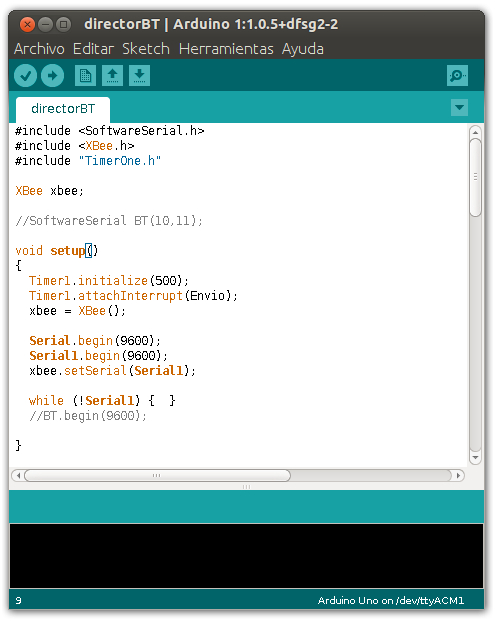
\includegraphics[width=0.6\textwidth]{./imagenes/arduinoide}
\caption{IDE Arduino} \label{fig:arduinoide}
\end{figure}


Justo debajo tenemos una serie de opciones (``Verificar", que compilará nuestro código; ``Cargar", que lo
subirá a nuestra placa Arduino; ``Nuevo", que creará un nuevo proyecto Arduino; ``Abrir", permite abrir un proyecto
Arduino ya cread; ``Guardar", para guardar el actual proyecto). A la derecha del todo, tenemos un monitor para el
puerto serial (para poder acceder a la comunicación entre nuestro equipo y la placa Arduino).\\

Si el lector no está familiarizado con el entorno y desea conocerlo algo más, puede consultar la bibliografía \cite{arduinoInicia} y
\cite{arduino24}.


\section{Actuador}
\title{Actuador}
Para que el músico sepa qué pulso es el correcto necesita alguna señal. Para ello
se ha decidido utilizar un micromotor vibrador. Para ser más exactos, el modelo 310-101 de la empresa
``Precision Microdrives" (figura \ref{fig:micromotor}).\\

\begin{figure}[!htb]
\centering
\captionsetup{justification=centering}
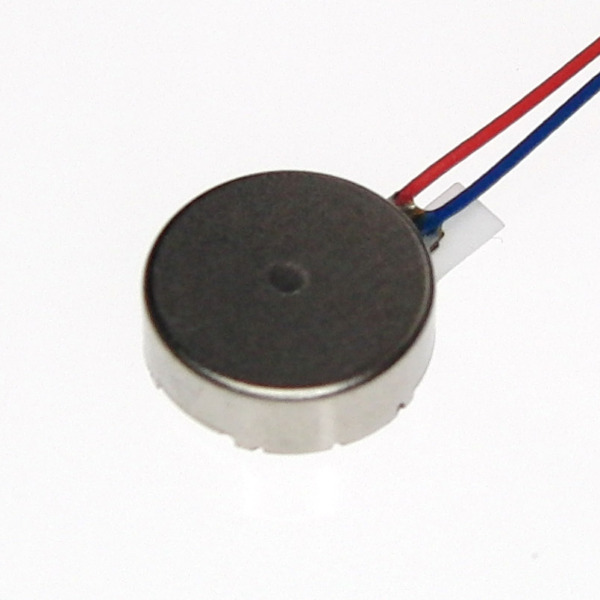
\includegraphics[width=0.5\textwidth]{./imagenes/micromotor}
\caption{Micromotor 310-101\\
\scriptsize{Imagen extraída de https://catalog.precisionmicrodrives.com}} \label{fig:micromotor}
\end{figure}


Sus características técnicas son:

\begin{itemize}
  \item Voltaje: 3V
  \item Diámetro: 10mm
  \item Longitud del cuerpo 3.4mm
  \item Peso: 1.2g
  \item Velocidad: 12000 rpm
  \item Intensidad: 85mA
  \item Resistencia: 75 Ohm
  \item Amplitud de vibración: 0,8G
\end{itemize}

Se puede consultar su datasheet en la bibliografía \cite{micromotorData}.



\section{Alimentación}
\title{Alimentación}

Gracias a la existencia de distintos tipos de placas Arduino, podemos crear dispositivos
con una forma u otra (como otro de los objetivos es la posibilidad de aumentar la funcionalidad
el sistema, habrá funcionalidades que necesiten de placas Arduino con un número distinto de
entradas/salidas al que se utilice aquí), aunque tendremos que intentar que sea lo más compacto
posible (para no ignorar aquel objetivo en el que se deseaba crear un sistema pequeño y discreto).\\

Por ejemplo, en caso que nos encontremos utilizando un Arduino Lilypad, la versión vestible de Arduino,
podremos elegir alguna de las opciones que se nos brindan para alimentar nuestro circuito, como el “LLYP-PSU”,
en el que podremos colocar una pila AAA o el “LilyPad 20mm Coin Cell Battery Holder”, para pilas de botón (cuyos
planos se encuentran disponibles en GitHub \cite{lilypadcoin}).\\

Otra opción a contemplar (y que cobrará mayor sentido al no usar la versión de Arduino vestible)
es la de utilizar bancos de energía (baterías externas). Estas baterías están pensadas para cargar
dispositivos móviles con gran consumo energético. La alta capacidad de estas baterías y el bajo consumo
de Arduino y XBee, tendrá como resultado la despreocupación del usuario en cuanto al plano energético.\\

Como se ha mencionado, en función del tipo de Arduino con el que construyamos nuestro ArduBand,
se seleccionará un tipo de alimentación u otra, quedando esto, generalmente, a opción del usuario
(sobre todo en el caso de la batería externa).\\

\section{Comunicación uno a muchos: estudio preliminar}
\title{Comunicación uno a muchos: estudio preliminar}

En los capítulos de \ref{cap:Diseno} y \ref{cap:Analisis} se ha ido viendo que es necesario
que un dispositivo emita un mensaje al resto de nodos de la red. Teniendo en cuenta que el
sistema se va a implementar como una red, la solución técnica que parece más adecuada
es realizar un \textit{broadcast} (un nodo envía una trama de datos a una dirección
especial, llamada dirección de broadcast, y todos los nodos reciben la trama de datos). Al querer
realizar una red con topología de estrella, es claro que el dispositivo central de
la red, y que interconecta al resto, será el que haga las veces de emisor.\\

ZigBee como tal permite conectar en estrella, malla o árbol. Según \cite{faludi} (tabla 1.1), se
puede configurar el XBee Series 2 (el que se está utilizando) para utilizar cualquiera de estar
topologías por defecto. Sin embargo no hay documentación sobre la forma de cambiar el comportamiento
por defecto (red de tipo malla).

En las redes formadas por dispositivos XBee tenemos tres tipos de dispositivos:
\begin{itemize}
  \item Coordinador: debe existir, al menos, uno por red. En caso de haber más, solo uno
  toma este rol (en caso de haber más de uno, se ponen de acuerdo y solo uno de ellos toma
  este rol, mientras que el otro pasa a ejercer de router). Se encarga de dirigir la red,
  estableciendo las rutas que deben seguir los paquetes. Puede comunicarse con todos los nodos
  \item Router: permite conectar nodos finales u otros routers con el coordinador. Puede
  comunicarse solo con el nodo coordinador (y sirve como puente para el traspaso de información
  entre el nodo coordinador y un nodo cualquiera)
  \item Dispositivo final: solo puede enviar información al coordinador (pudiendo utilizar
  los routers para hacer llegar la trama hasta su destino). Pasan la mayor parte del tiempo
  durmiendo, es decir, en un estado de bajo consumo energético
\end{itemize}

\begin{figure}[!htb]
\centering
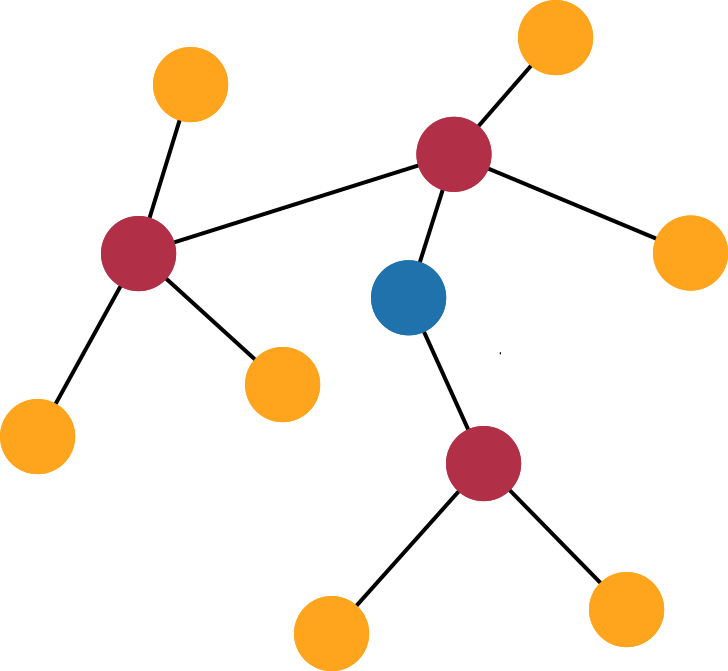
\includegraphics[width=0.6\textwidth]{./imagenes/mesh}
\caption{Red de tipo \textit{mesh}} \label{fig:mesh}
\end{figure}

En la figura \ref{fig:mesh} podemos ver un ejemplo de red XBee ZigBee.
\begin{itemize}
  \item  \textcolor{blueS}{$\blacksquare$} Coordinador
  \item  \textcolor{rojoOscuroS}{$\blacksquare$} Router
  \item  \textcolor{naranjaS}{$\blacksquare$} Dispositivo final
\end{itemize}

Teniendo en cuenta los tipos de nodos que tenemos, podemos crear una topología en estrella
(la que más encaja con nuestro proyecto) a partir de la topología en malla: no tendremos
disposivios de tipo router. De esta forma evitaremos que haya saltos intermedios entre
el dispositivo final (músico) y el director.\\

Esto puede parecer un inconveniente en bandas largas (no disponemos de routers
que hagan de puente con dispositivos finales que se encuentren demasiado lejos)
pero si volvemos a mirar la tabla 1.1 de \cite{faludi}, veremos que el rango
de alcance se sitúa entre los 40 y 120 metros. Teniendo en cuenta que en la
formación de una banda de música la separación entre dos filas de músicos es de
1 metro aproximadamente, en el peor de los casos, estaríamos llegando a 80 metros
(si situamos el dispositivo en el centro de la banda). Si establecemos una media de
4 músicos por fila, en una banda de 80 metros de largo tendríamos 320 músicos.
Teniendo en cuenta que la banda de la que se hablaba en la introducción \cite{cigarreras}
es una de las más numerosas con alrededor de 140 músicos, es claro que esto no es
un problema.\\

\subsection{Problema en broadcast}
\title{Problema en broadcast}

En el apartado anterior se explicaba que la solución que parece más directa es realizar
un \textit{broadcast}. Pero es una idea que se desecha rápidamente al hacer el siguiente experimento:

\begin{enumerate}
  \item Se configura una mota como coordinador (instalándo el firmware oportuno, eligiendo el modo API)
  \item A esta mota se le inserta la dirección de \textit{broadcast} como
  dirección de destino (0x0 para la DH y 0xFFFF para DL)
  \item Se le inserta un \textit{PAN ID}
  \item Se configura otra mota como dispositivo final (con firmware en modo API
  y con el mismo \textit{PAN ID})
  \item Pulsamos sobre el menú para controlar el puerto serial (en la mota coordinadora)
  (la descrita en la figgura \ref{fig:interfaz2})
  \item Creamos un paquete con un solo carácter y ponemos que se envíe infinitas veces
  cada 500ms
  \item Comprobamos, en el dispositivo final, la traza y comprobamos lo tiempos
\end{enumerate}

El configurar ambas motas en modo API es por los siguientes motivos:
\begin{itemize}
  \item Nodo final: XCTU muestra el tiempo de llegada de los paquetes. En modo AT
    (transparente), no
  \item Nodo director: para poder modificar los datos del paquete
\end{itemize}

Este experimento se ha realizado varias veces. Un ejemplo de lo que ocurre se muestra
en la figura \ref{fig:pruebasxctu_broadcast}. En la figura \ref{fig:graficabroadcast}
se muestra de una forma distinta la misma información (el eje X está en segundos y en
el eje Y se muestra la llegada de un paquete).\\

\begin{figure}[!htb]
\centering
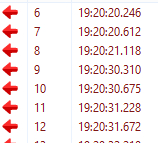
\includegraphics[width=0.4\textwidth]{./imagenes/pruebasxctu_broadcast}
\caption{Traza temporal de llegada de paquetes en X-CTU con \textit{broadcast}} \label{fig:pruebasxctu_broadcast}
\end{figure}


\begin{figure}[!htb]
\centering
\captionsetup{justification=centering}
\begin{tikzpicture}
\draw[latex-latex, thin, draw=gray] (-1,0)--(12,0) node [right] {$x$};
\draw[latex-latex, thin, draw=gray] (0,-1)--(0,4) node [above] {$y$};

\foreach \Point in { (0.246,3),(0.612,3),(1.118,3),(10.310,3),(10.675,3),(11.228,3),(11.672,3) }{
   \node at \Point {\textbullet};
}

\draw [blue,solid] (0,0) -- (0.246,3);
\draw [blue,solid] (0.246,3) -- (0.246,0);
\draw [blue,solid] (0.246,0) -- (0.612,3);
\draw [blue,solid] (0.612,3) -- (0.612,0);
\draw [blue,solid] (0.612,0) -- (1.118,3);
\draw [blue,solid] (1.118,3) -- (1.118,0);
\draw [blue,solid] (1.118,0) -- (10.310,0);
\draw [blue,solid] (10.160,0) -- (10.310,3);
\draw [blue,solid] (10.310,3) -- (10.310,0);
\draw [blue,solid] (10.310,0) -- (10.675,3);
\draw [blue,solid] (10.675,3) -- (10.675,0);
\draw [blue,solid] (10.675,0) -- (11.228,3);
\draw [blue,solid] (11.228,3) -- (11.228,0);
\draw [blue,solid] (11.228,0) -- (11.672,3);

\draw [dotted, gray] (-1,-1) grid (12,5);

\foreach \x in {0,1,2,3,4,5,6,7,8,9,10,11,12}
    \draw (\x cm,1pt) -- (\x cm,-1pt) node[anchor=north] {$\x$};

\node[draw] at (-1,3) {INPUT};
\end{tikzpicture}


\caption{Representación temporal de la llegada de paquetes utilizando \textit{broadcast}\\
 (X está en segundos)} \label{fig:graficabroadcast}
\end{figure}

Aunque parece al principio que la recepción de paquetes es regular, después hay un largo
periodo de tiempo (unos 9 segundos) donde no se recibe nada.\\

Si modificamos el paquete en el nodo director para que no envíe ACK de la capa de
aplicación (que podría ser el culpable), se obtienen similares resultados. Para modificar el paquete simplemente
hay que crearlo de la misma forma que antes y, en el editor de paquetes que provee XCTU
(en el mismo lugar donde se crean), se cambia el segundo \textit{byte} de la traza por 0. Si
por ejemplo tenemos el siguiente paquete:  \texttt{7E 01 0F 90 00 7D 33 A2 00 40 A0 9B EC 00 00 01 78 DC},
deberemos convertirlo en este otro  \texttt{7E 00 0F 90 00 7D 33 A2 00 40 A0 9B EC 00 00 01 78 DC}
(solo cambia el segundo \textit{byte}).

Este problema podríamos achacarlo a la capa firmware de la mota (que podría contener mecanismos
para comprobar la integridad de los paquetes y evitar que lleguen trazas corruptas).
Sin embargo, es demasiado tiempo como para que este sea el problema (además, en una comunicación \text{unicast}
(con un solo nodo), el problema no existe -como podemos ver en la figura \ref{fig:xctu_comunicacionunoauno}- y en la gráfica
\ref{fig:graficaunicast}, ya que la tasa de llegada de paquetes se mantiene constante -aproximadamente-).

\begin{figure}[!htb]
\centering
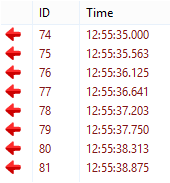
\includegraphics[width=0.4\textwidth]{./imagenes/xctu_comunicacionunoauno}
\caption{Traza temporal de llegada de paquetes en X-CTU con \textit{unicast}} \label{fig:xctu_comunicacionunoauno}
\end{figure}


\begin{figure}[!htb]
\centering
\captionsetup{justification=centering}
\begin{tikzpicture}
\draw[latex-latex, thin, draw=gray] (-1,0)--(6,0) node [right] {$x$};
\draw[latex-latex, thin, draw=gray] (0,-1)--(0,4) node [above] {$y$};

\foreach \Point in { (0,3),(0.563,3),(1.125,3),(1.641,3),(2.203,3),(2.750,3),(3.313,3),(3.875,3) }{
   \node at \Point {\textbullet};
}

\draw [blue,solid] (0,0) -- (0,3);
\draw [blue,solid] (0,3) -- (0.2,0);
\draw [blue,solid] (0.2,0) -- (0.563,3);
\draw [blue,solid] (0.563,3) -- (0.563,0);
\draw [blue,solid] (0.563,0) -- (1.125,3);
\draw [blue,solid] (1.125,3) -- (1.125,0);
\draw [blue,solid] (1.125,0) -- (1.641,3);
\draw [blue,solid] (1.641,3) -- (1.641,0);
\draw [blue,solid] (1.641,0) -- (2.203,3);
\draw [blue,solid] (2.203,3) -- (2.203,0);
\draw [blue,solid] (2.203,0) -- (2.750,3);
\draw [blue,solid] (2.750,3) -- (2.750,0);
\draw [blue,solid] (2.750,0) -- (3.313,3);
\draw [blue,solid] (3.313,3) -- (3.313,0);
\draw [blue,solid] (3.313,0) -- (3.875,3);
\draw [blue,solid] (3.875,3) -- (3.875,0);

\draw [dotted, gray] (-1,-1) grid (6,5);

\foreach \x in {0,1,2,3,4,5}
    \draw (\x cm,1pt) -- (\x cm,-1pt) node[anchor=north] {$\x$};

\node[draw] at (-1,3) {INPUT};
\end{tikzpicture}

\caption{Representación temporal de la llegada de paquetes utilizando \textit{unicast}\\
(X está en segundos)} \label{fig:graficaunicast}
\end{figure}

Cabe destacar que se recibe un paquete más en menos tiempo.\\

El problema viene por la forma en la que está implementado el \textit{broadcast}:
los nodos se encuentran en una topología de malla y, cada vez que reciben un broadcast,
lo repiten hasta tres veces. Esto no sería un problema si no fuera por que la red
permite un número máximo de broadcast a la vez. Al llegar a ese límite, la mota
coordinadora deja de poder seguir enviando paquetes (no solo hasta que terminen los
\textit{broadcast} existentes, sino hasta que cada mota termine de reenviar 3 veces
cada uno de los paquetes que ha recibido). Es por eso que ha tenido que pasar un tiempo
hasta que la red se sature. Si esto ha pasado con un solo nodo receptor, el problema
se agravaría cuanto mayor fuese la cantidad de nodos en la red. \\

En otras versiones de la mota existe la posibilidad de crear un \textit{multicast},
pero no en esta, por lo que no es una solución viable.\\

La solución que se propone es enviar individualmente a cada dispositivo el paquete, es decir,
hacer un \textit{broadcast} a base de \textit{unicast}. Facilitar esta tarea, es mejor
utilizar el modo API (en el modo AT se puede, pero habría que estar entrando constantemente
al modo comando y, a veces, cuando se entra en este modo, la mota necesita ser reinicia -y,
al no poder reiniciarla, dejaría de funcionar ese nodo-.)\\

Nace ahora una nueva contrariedad: existe un retardo inevitable (de unos pocos milisegundos)
cada vez que se envía un paquete. Entre dos envíos no es problema ya que, cuando
se sincronicen los nodos, los músicos no notarán diferencia. Cuando se envíen 50, sí lo será.\\

Supongamos que hay 50 músicos y cada envío produce un retardo de 15ms. Cuando se llegue al músico
50, habrá habido 49 envíos, luego:
\[
  49 \times 15 = 735ms
\]

Es un retardo de casi un segundo. Como remedio, se propone lo siguiente: en vez de
sincronizar siempre todos los nodos, se sincronizan por turnos. Para entenderlo mejor se
va a recurrir a un poco de notación musical. En la introducción se vió el concepto de \textit{compás}
(una forma de separar los pentagramas para facilitar la lectura de la música). En el desarrollo
del proyecto, se ha tomado que los compases son de 4/4 (esto significa que en un compás se pueden introducir
cuatro notas negras, que tienen un pulso cada una, es decir, que por cada compás,
habrá cuatro pulsos). Entoncesen vez de sincronizar a todos los músicos en todos los pulsos,
a cada pulso se puede sincronizar un músico y su dispositivo, internamente, que mantenga el tempo hasta
que reciba otra señal desde el nodo del director. Esta división puede entenderse mejor viendo
la figura \ref{fig:sincronotas} donde se sincroniza a un músico distinto en cada pulso.

\begin{figure}[!htb]
\centering
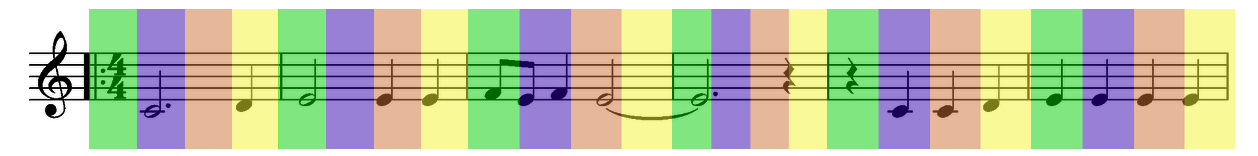
\includegraphics[width=1\textwidth]{./imagenes/sincronotas}
\caption{Sincronización en cada pulso a un músico diferente} \label{fig:sincronotas}
\end{figure}

En la figura \ref{fig:sincronotas} se está sincronizando a un músico por pulso. En
la figura del ejemplo habría cuatro músicos (por eso hay cuatro colores).\\

Al sincronizarse a un músico en cada pulso y que él mantenga el mismo tempo que los demás,
la sincronización no se pierde (salvo que, por algún motivo), una recepción tarde más de
la cuenta.\\

Esto tal vez haga que la red tenga demasiadas tareas y la fiabilidad disminuya. Para
cubrir este aspecto, no se sincroniza en cada pulso, si no en cada compás (como hay
cuatro pulsos en cada compás, las comunicaciones se reducen a una cuarta parte).
En la figura \ref{fig:sincrocompas} se puede ver de forma gráfica.\\

\begin{figure}[!htb]
\centering
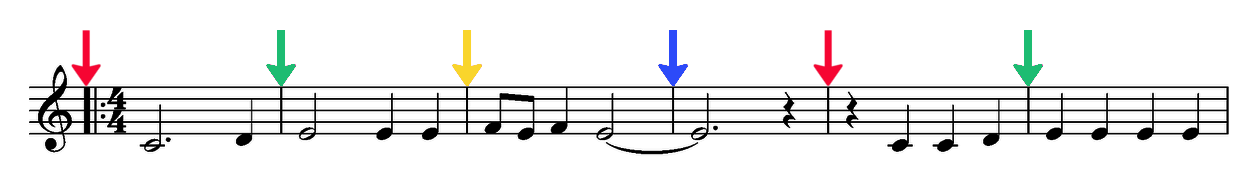
\includegraphics[width=1\textwidth]{./imagenes/sincrocompas}
\caption{Sincronización en cada compás a un músico diferente} \label{fig:sincrocompas}
\end{figure}

Cada flecha de un color es un músico sincronizado. Al igual que en el ejemplo anterior,
deberá mantener el tempo de forma local, hasta que llegue otra señal por parte del director.\\

Que el director envíe constantemente el pulso permite que, en caso que uno de los
paquetes haya llegado más tarde de la cuenta, se pueda corregir.\\

Para comprobar que funciona, se hace un experimento similar al de los casos anteriores pero,
esta vez, midiendo tiempos en dos dispositivos receptores.

\begin{figure}[!htb]
\centering
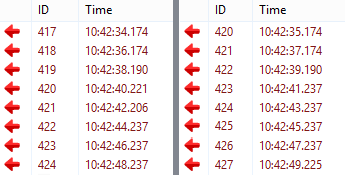
\includegraphics[width=0.7\textwidth]{./imagenes/sincronizacion}
\caption{Sincronización en cada compás a un músico diferente} \label{fig:sincronizacion}
\end{figure}



  \begin{figure}[!htb]
  \centering
  \captionsetup{justification=centering}
  \resizebox{0.9\textwidth}{!}{
  \begin{tikzpicture}
  \draw[latex-latex, thin, draw=gray] (-1,0)--(6,0) node [right] {$x$};
  \draw[latex-latex, thin, draw=gray] (0,-1)--(0,4) node [above] {$y$};


%Primero el izquierdo
  \foreach \Point in {(0.174,3),(2.174,3),(4.190,3),(6.221,3),(8.206,3),(10.237,3),
  (12.337,3),(14.237,3)}{
     \node at \Point {\textbullet};
  }

  \draw [blue,solid] (0,0) -- (0.174,3);
  \draw [blue,solid]  (0.174,3) -- (0.174,0);
  \draw [blue,solid]  (0.174,0) -- (2.174,3);
  \draw [blue,solid]  (2.174,3) -- (2.174,0);
  \draw [blue,solid]  (2.174,0) -- (4.190,3);
  \draw [blue,solid]  (4.190,3) -- (4.190,0);
  \draw [blue,solid]  (4.190,0) -- (6.221,3);
  \draw [blue,solid]  (6.221,3) -- (6.221,0);
  \draw [blue,solid]  (6.221,0) -- (8.206,3);
  \draw [blue,solid]  (8.206,3) -- (8.206,0);
  \draw [blue,solid]  (8.206,0) -- (10.237,3);
  \draw [blue,solid]  (10.237,3) -- (10.237,0);
  \draw [blue,solid]  (10.237,0) -- (12.337,3);
  \draw [blue,solid]  (12.337,3) -- (12.337,0);
  \draw [blue,solid]  (12.337,0) -- (14.237,3);

%Ahora el derecho
\foreach \Point in {(1.174,3),(3.174,3),(5.190,3),(7.237,3),(9.237,3),(11.237,3),(13.237,3),(15.225,3)}{
   \node at \Point {\textbullet};
}

\draw [red,solid] (0,0) -- (1.174,3);
\draw [red,solid] (1.174,3) -- (1.174,0);
\draw [red,solid] (1.174,0) -- (3.174,3);
\draw [red,solid] (3.174,3) -- (3.174,0);
\draw [red,solid] (3.174,0) -- (5.190,3);
\draw [red,solid] (5.190,3) -- (5.190,0);
\draw [red,solid] (5.190,0) -- (7.237,3);
\draw [red,solid] (7.237,3) -- (7.237,0);
\draw [red,solid] (7.237,0) -- (9.237,3);
\draw [red,solid] (9.237,3) -- (9.237,0);
\draw [red,solid] (9.237,0) -- (11.237,3);
\draw [red,solid] (11.237,3) -- (11.237,0);
\draw [red,solid] (11.237,0) -- (13.237,3);
\draw [red,solid] (13.237,3) -- (13.237,0);
\draw [red,solid] (13.237,0) -- (15.225,3);


  \draw [dotted, gray] (-1,-1) grid (18,5);

  \foreach \x in {0,1,2,3,4,5,6,7,8,9,10,11,12,13,14,15,16,17}
      \draw (\x cm,1pt) -- (\x cm,-1pt) node[anchor=north] {$\x$};

  \node[draw] at (-1,3) {INPUT};
  \end{tikzpicture}
  }


  \caption{Representación temporal de la llegada de paquetes utilizando \textit{unicast}\\
  (X está en segundos)} \label{fig:graficasincronizados}
  \end{figure}

Como se puede ver en \ref{fig:sincronizacion} y \ref{fig:graficasincronizados},
la sincronización que se ha obtenido es bastante buena. Cada uno de los dispositivos
es sincronizado cada un segundo (por eso, si miramos una de las trazas,
vemos que hay en torno a dos segundo de espera entre la llegada de un paquete y otro
-1 segundo para sincronizar al otro XBee y 1 para sincronizar al que estamos monitorizando-).\\

Si examinamos las trazas, se observa cómo hay, en algunas ocasiones, sincronización
a nivel de milisegundos. También es interesante ver que en muchas ocasiones (como en los
paquetes de la traza de la derecha con ID comprendidas entre 423 y 426 -inclusive-) la
llegada de paquetes es en el mismo milisegundo de segundos distintos, por ejemplo: en el
momento 10:42:45.237 (ID:425) y 10:42:47.237 (ID:426). Cuando esto no ocurre, el error es asumible.\\



\section{Modalidades del dispositivo}
\title{Modalidades del dispositivo}

Tras el análisis realizado sobre la estructura de la red, toca hablar de los dos tipos
de nodos de los que se disponen: director y músico.

\subsection{El dispositivo director}
\title{El dispositivo director}

El dispositivo del director tiene que comunicarse con el resto de dispositivos (los
de los músicos) y con el dispositivo Android. Para enlazar con los otros músicos
se va a utilizar la red inalámbrica de sensores mientras que, para la conexión
con el dispositivo Android se ha elegido utilizar Bluetooth (HC05 \cite{bthc05}) ya que es un sistema
de comunicación que tienen todos los dispositivos móviles (tanto \textit{tablets} como
\textit{smartphones}). Además (ya se estudió al principio de este capítulo), la versión
4 de Bluetooth tiene mecanismos para ahorro de energía (y como la comunicación va a durar
poco tiempo, no se necesita más).\\


\subsection{Controlador del dispositivo director}
\title{Controlador del dispositivo director}

Para llevar a cabo todo el proceso que se ha ido describiendo, es necesario programar
la placa Arduino. Teniendo en cuenta que hay que cumplir unos requisitos de tiempo bastante
fuertes, se ha elegido trabajar con timers. Arduino cuenta con dos timers: uno reservado
a la ejecución del propio código y otro que puede ser utilizado por el desarrollador.
La biblioteca ``Timer1" \cite{timeronearduino} facilita la manipulación de esta característica.\\

Por otra parte, es necesaria la utilización de dos puertos serial (uno pra XBee y otro para el Bluetooth).
La mayoría de versiones de Arduino (Lilypad, por ejemplo), no tienen más de un puerto.
Por ello se utiliza la biblioteca ``Software Serial" \cite{softwareserial} que, mediante software, consigue
que unos puertos que no son puerto serial, actúen como tal.\\

A continuación se muestra un pseudocódigo de lo que se ha implementado.\\
\floatname{algorithm}{Algoritmo}
\begin{algorithm}
  \begin{algorithmic}[1]
     \State $tiempo\gets 0$
     \State $i\gets 0$
     \State $leer \gets true$\\

     \Function{Envio}{}
      \If {$ahora - i\geq periodo $}
        \State enviarPaquete($i$)
        \State $i \gets i+1(mod(numeroXBee))$
        \State $tiempo \gets ahora$
      \EndIf
      \EndFunction\\

    \While{true}
    \If{$leer$}
      \If{Hay datos del Bluetooth}
        \State $leer \gets false$
        \State $tiempo\gets tiempoEntrePulso(leerBluetooth())*4$
        \State Se generan los paquetes
        \State Se inicia el timer con la funcion envio
      \EndIf
     \EndIf
    \EndWhile
  \caption{Algoritmo utilizando por el controlador del director}
  \end{algorithmic}
\end{algorithm}



\begin{enumerate}
  \item Se declara la función que ejecutará el timer. Esta función comprueba cuánto
   tiempo ha pasado desde la última vez que se ejecutó
    \begin{itemize}
      \item Si ha pasado suficiente, enviará un mensaje al nodo que le toque sincronizar
    \end{itemize}
  \item En el bucle que se ejecuta continuamente, si leer(*) es verdadero:
    \begin{enumerate}
      \item Se lee del Bluetooth el tempo y se generan los paquetes para cada dirección XBee
      \item Se calculan los pulsos por segundo, después el tiempo entre pulso y se multiplica
      por 4 (para sincronizar cada 4 pulsos, es decir, cada compás de 4/4)
      \item Se generan los paquetes a enviar
      \item Se activa el timer (cada medio milisegundo para mantenerlo en activo -aunque haya momentos que se llame
      al timer para nada, esto provoca que sea más preciso que si lo ajustásemos al tiempo entre pulsos y, de todas formas,
      va a quedar en el bucle de espera activa, la función ``loop"-).
    \end{enumerate}
\end{enumerate}

Lo que se acaba de explicar es el algoritmo. En la implementación en Arduino, se necesitan
declarar los pines, inicializar algunas variables... También se desactiva el Bluetooth para
ahorrar energía.\\

(*)Esta variable ``leer"\ permite que, una vez que se apaga el Bluetooth, no se vuelva a intentar leer
(ya que no se conseguirán datos -y la lectura de serial es más lenta- o estos serán erróneos
-lo que nos llevará a un fallo en el sistema-).\\


\subsection{Esquema de conexionado del dispositivo director}
\title{Esquema de conexionado del dispositivo director}

Este esquema se puede consultar en la figura \ref{fig:director_esquema}. Falta
la mota XBee, que iría sobre la shield, y la alimentación que se realizaría mediante un
dispositivo FTDI-USB.\\

\begin{figure}[!htb]
\centering
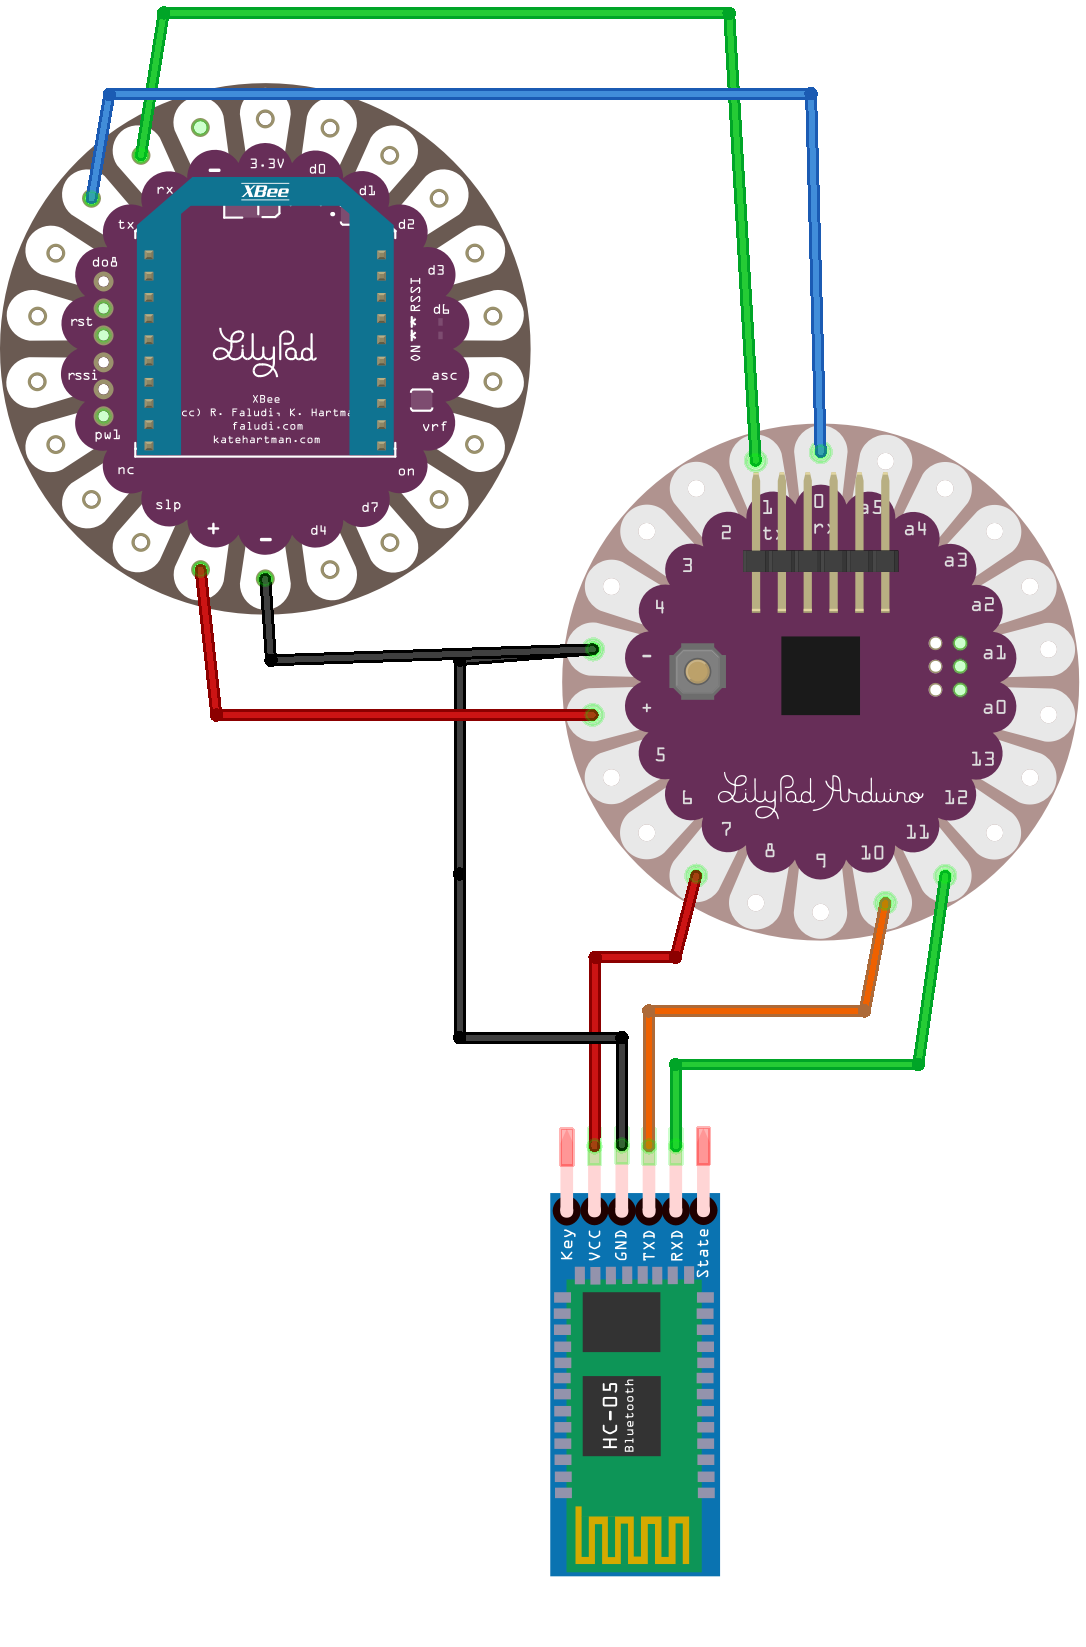
\includegraphics[width=1\textwidth]{./imagenes/director_esquema}
\caption{Esquema de conexionado del director} \label{fig:director_esquema}
\end{figure}

\clearpage

\section{Carcasa}
\title{Carcasa}

La carcasa que se propone tiene dos partes:
\begin{itemize}
  \item Base: dentro de esta parte van todos los componentes. En la parte inferior pone ``Director"
  para poder diferenciarlo de los dispositivos de los músicos
  \item Tapa: permite dejar todos los componentes dentro para que no se salgan. LLeva el logotipo
  de ArduBand. Se une a la base utilizando algún adhesivo.
\end{itemize}

El hueco que queda libre es para colocar ahí la salida a MiniUSB del FTDI (para conectar la alimentación).\\

\begin{figure}[!htb]
\centering
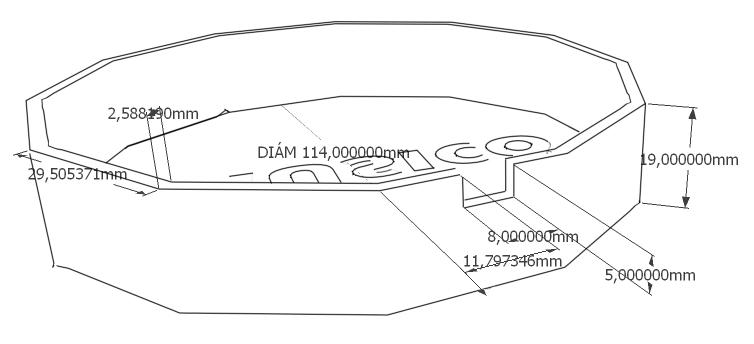
\includegraphics[width=1\textwidth]{./imagenes/carcasa_base}
\caption{Base de la carcasa} \label{fig:carcasa_base}
\end{figure}

\begin{figure}[!htb]
\centering
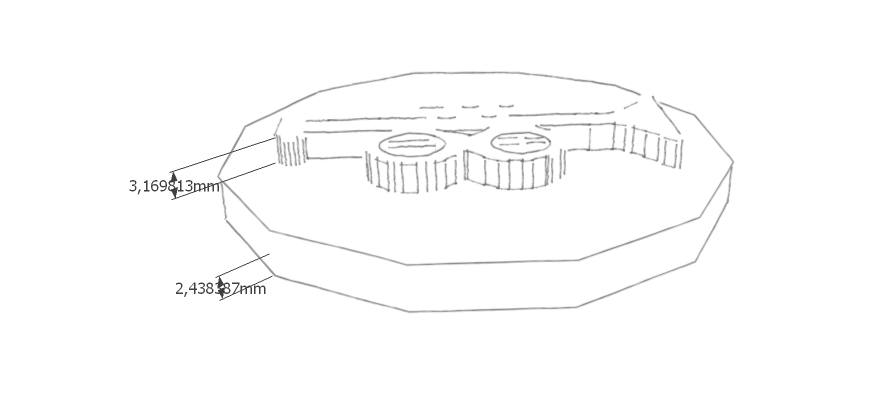
\includegraphics[width=1\textwidth]{./imagenes/carcasa_tapa}
\caption{Tapa de la carcasa} \label{fig:carcasa_tapa}
\end{figure}

\begin{figure}[!htb]
\centering
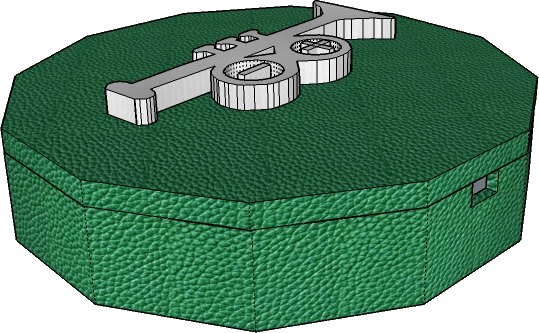
\includegraphics[width=1\textwidth]{./imagenes/carcasa_modelo}
\caption{Modelo 3D de la carcasa} \label{fig:carcasa_modelo}
\end{figure}

%
%\input{capitulos/08_Pruebas}
%
%\input{capitulos/09_Conclusiones}
%
%\input{capitulos/10_Conclusiones y trabajos futuros}
%%\chapter{Conclusiones y Trabajos Futuros}
%
%
\nocite{*}
\bibliography{bibliografia}\addcontentsline{toc}{chapter}{Bibliografía}
\bibliographystyle{unsrt}
%
%\appendix
%\input{apendices/manual_usuario/manual_usuario}
%%\input{apendices/paper/paper}
%\input{glosario/entradas_glosario}
% \addcontentsline{toc}{chapter}{Glosario}
% \printglossary

\addcontentsline{toc}{chapter}{Lista de figuras}
\listoffigures

\chapter*{}
\thispagestyle{empty}

\end{document}
